\documentclass[10pt,twocolumn,letterpaper]{article}
\usepackage{wacv,times,epsfig,graphicx,amsmath,amssymb}
\usepackage{caption,subcaption,multirow,bigstrut,paralist}


\usepackage[pagebackref=false,breaklinks=true,letterpaper=true,colorlinks,bookmarks=false]{hyperref}

\newcommand{\todo}[1]{\textcolor{red}{todo: {\em #1}}}
\newcommand{\figref}[1]{Figure~\ref{fig:#1}}
\newcommand{\tblref}[1]{Table~\ref{tbl:#1}}

\wacvfinalcopy % *** Uncomment this line for the final submission

\def\wacvPaperID{20} % *** Enter the wacv Paper ID here
\def\httilde{\mbox{\tt\raisebox{-.5ex}{\symbol{126}}}}

% Pages are numbered in submission mode, and unnumbered in camera-ready
\ifwacvfinal\pagestyle{empty}\fi
\setcounter{page}{1}


\begin{document}


%\title{Deep Methods for Estimating Transient Scene Properties}
\title{A Fast Method for Estimating Transient Scene Attributes}


\author{Ryan Baltenberger, Menghua Zhai, Connor Greenwell, Scott Workman, Nathan Jacobs \\
  Department of Computer Science, University of Kentucky \\
  {\tt\small \{rbalten, ted, connor, scott, jacobs\}@cs.uky.edu}
}

\maketitle
\ifwacvfinal\thispagestyle{empty}\fi


\begin{abstract}

We propose the use of deep convolutional neural networks to estimate the
transient attributes of a scene from a single image.  Transient scene
attributes describe both the objective conditions, such as the weather, time of
day, and the season, and subjective properties of a scene, such as whether or
not the scene seems busy. Recently, convolutional neural networks have been
used to achieve state-of-the-art results for many vision problems, from object
detection to scene classification, but have not previously been used for
estimating transient attributes. We compare several methods for adapting an
existing network architecture and present state-of-the-art results on two
benchmark datasets. Our method is more accurate and significantly faster than
previous methods, enabling real-world applications. 

\end{abstract}

\section{Introduction}
% general intro to the problem and why it is important
Outdoor scenes experience a wide range of lighting and weather conditions which
dramatically affect their appearance. A scene can change from rainy and
brooding to sunny and pleasant in a matter of hours, even minutes. The ability
to quickly understand these fleeting, or transient, attributes is a critical
skill that people often take for granted. Automatically understanding such
subtle conditions has many potential applications, including: improving
context-dependent anomaly detection~\cite{abrams12lost}; enabling
attribute-oriented browsing and search of large image
sets\cite{jacobs07amos,skyfinder}; estimating micro-climate conditions using
outdoor webcams~\cite{islam13webcamweather}; as a pre-processing step for
higher-level algorithms for
calibration~\cite{jacobs13cloudcalibration,workman2014rainbow}, shape
estimation~\cite{abramsheliometric,workman2015distributed},
geolocalization~\cite{jacobs07geolocate}; and  environmental
monitoring~\cite{jacobs09webcamgis}. 

% what do we propose to do? 

We propose a fast method for predicting transient attributes from a single
image using deep convolutional neural networks (CNNs). CNNs have been used to
obtain state-of-the-art results for many vision tasks, including object
classification~\cite{krizhevsky2012imagenet}, object
detection~\cite{girshick2013rich}, and scene
classification~\cite{zhou2014places} but have not been used to estimate
transient scene attributes. Our work addresses two specific problems related to
estimating transient scene attributes. First, the problem of estimating whether
it is sunny or cloudy~\cite{lutwoclass} and second, predicting the degree to
which various transient attributes are present in the scene~\cite{Laffont14}.
To this end, we present two different networks and three different training
initializations. Our methods achieve state-of-the-art results on two benchmark
datasets and are significantly faster than previous approaches.
\figref{cartoon} shows an overview of our method.  

%Input images are pushed through the specially trained
%CNN that outputs a set of attribute values.

%\figref{results} shows the output of our
%methods for several example images.

\begin{figure}[t]
	\centering
		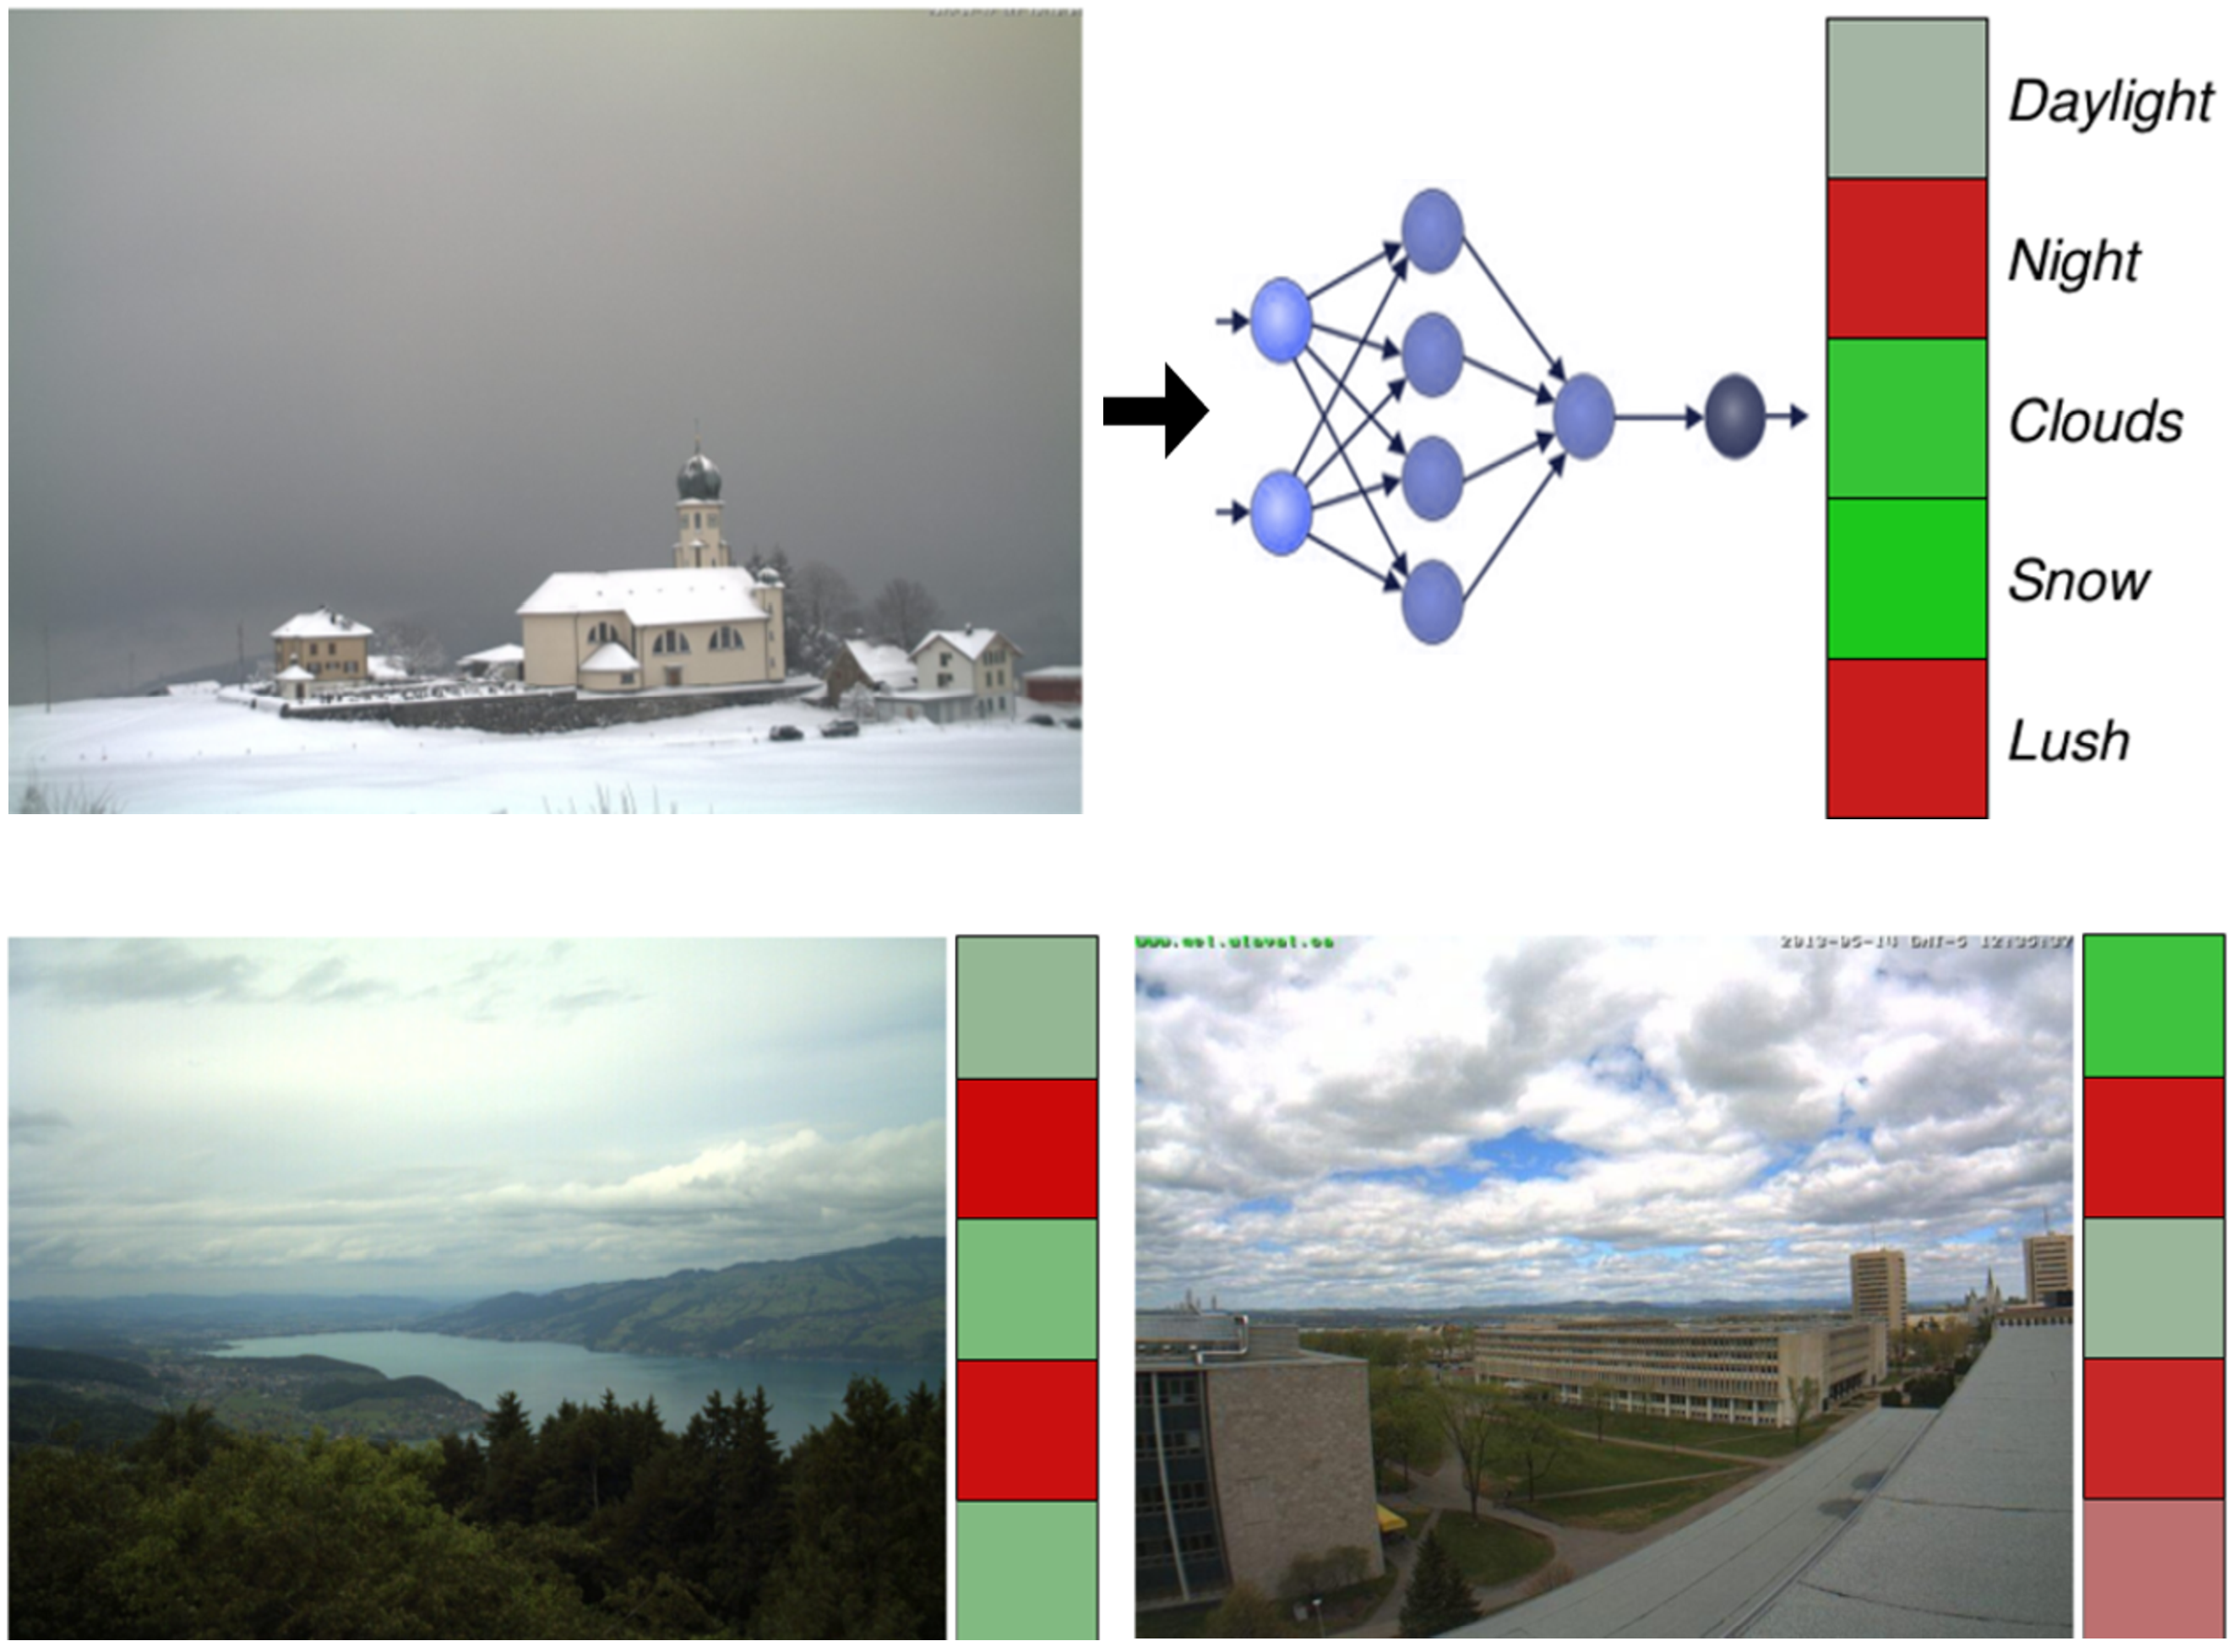
\includegraphics[width=\linewidth, trim= 0mm 0mm 0mm 0mm]{figs/cartoon.pdf}
    \caption{Our method predicts transient scene attributes from a
      single image using a deep convolutional neural network. For a
      subset of attributes, the predicted values (green=attribute
      present, gray=uncertain, red=attribute absent) are shown for
      three example images. 
    }
      %This shows an overview of our proposed method and a subset of the
      %       output attributes.  In this case, red is a low attribute value and
      %       green is a high attribute value.
		\label{fig:cartoon}
\end{figure}

%\begin{figure}
%	\centering
%		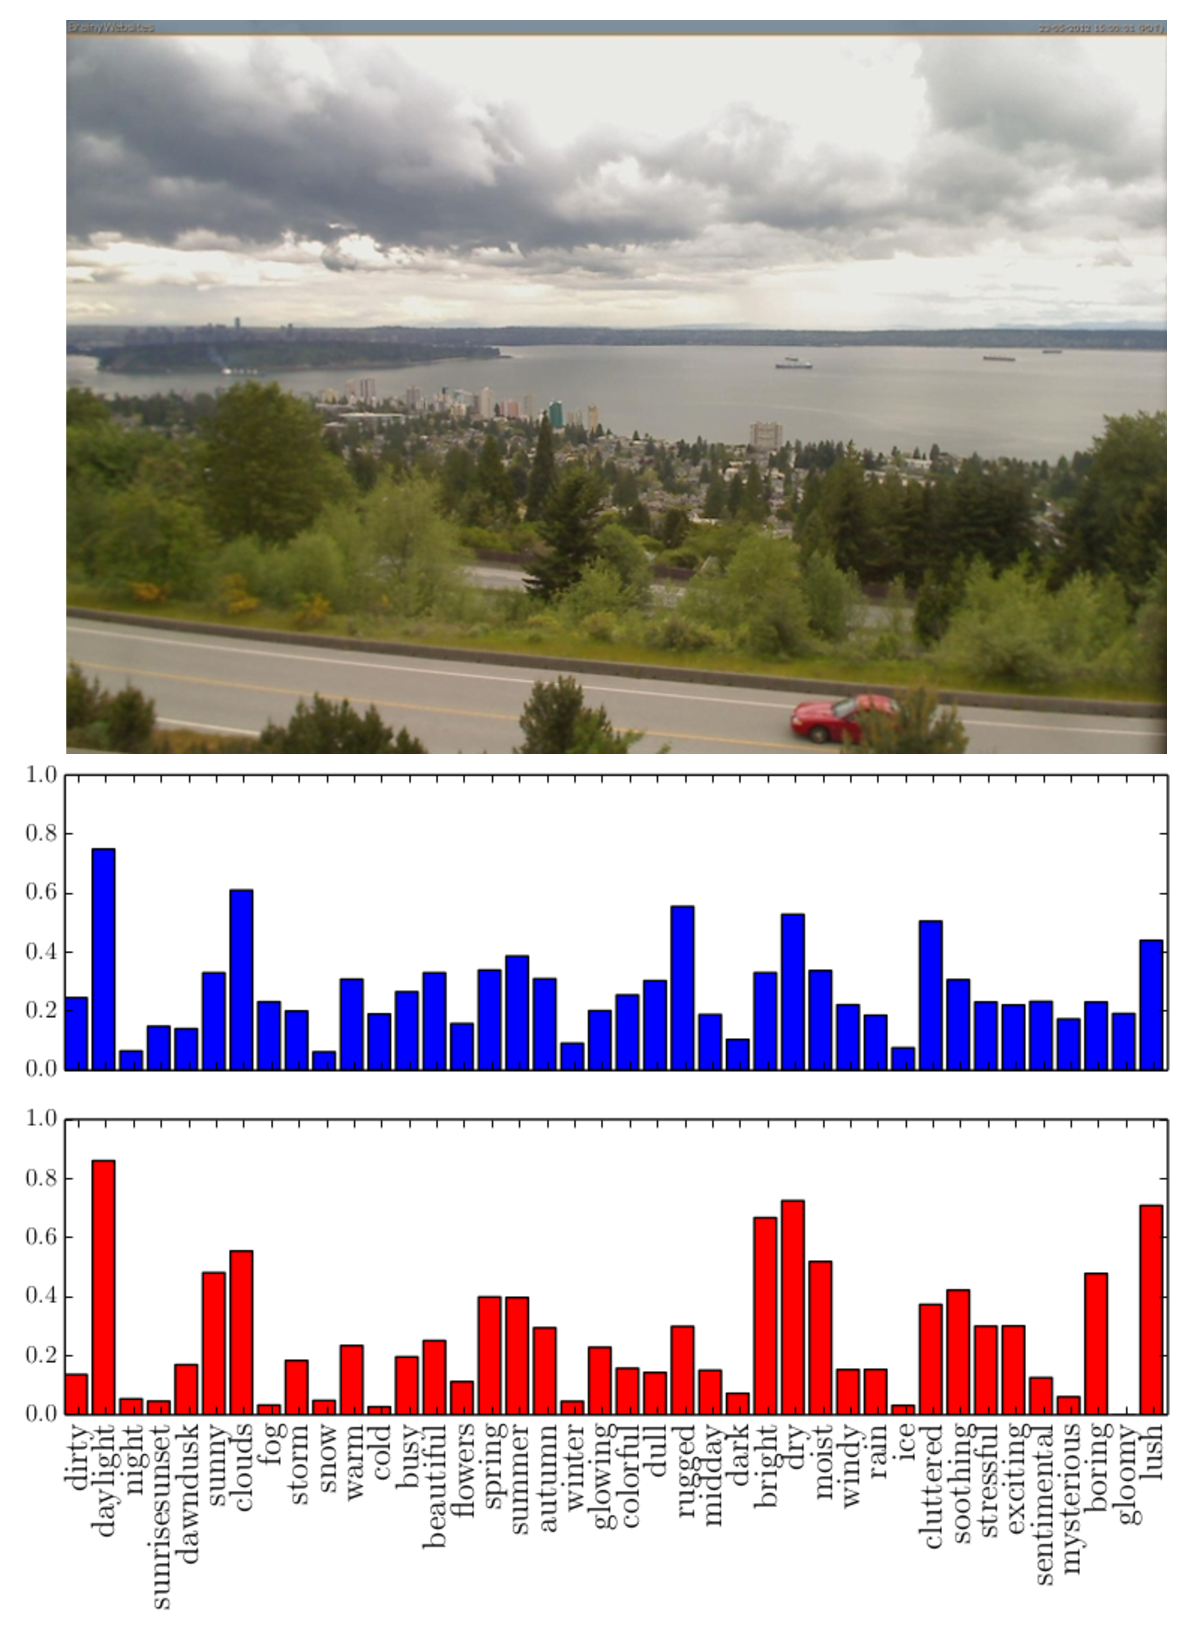
\includegraphics[width=0.5\textwidth]{figs/bars.pdf}
%		\caption{Example images from the Transient Attributes Dataset
%      with our network's confidence in each predicted label.
%      \todo{boring}}
%    \label{fig:results}
%\end{figure}

% what we can do now that we have this?

The key contributions of this work are: 1) proposing several CNN
training initializations for predicting transient attributes, 2) evaluating
the proposed methods on two benchmark datasets, 3) releasing
pre-trained networks for classifying transient scene attributes in a
popular deep learning framework, and 4) demonstrating several
applications of the networks to webcam image understanding. 

\subsection{Related Work}
Attributes are high-level descriptions of a visual property which offer some
additional semantic context for understanding an object, activity, or scene.
For example, a \emph{green} apple or a \emph{cloudy} day. Representations based
on such visual attributes have become increasingly popular in the vision
community as they offer the ability to to generalize across categories. The
first learning-based methods to take advantage of such high-level attributes
arose for the task of object
recognition~\cite{farhadi2009describing,lampert2009learning}, demonstrating the
power of learning by description. Many methods were quick to follow suit, with
applications ranging from content-based image
retrieval~\cite{siddiquie2011image} to characterizing facial
appearance~\cite{kumar2011describable}. Given their prowess, a significant
amount of research has focused on identifying useful
attributes~\cite{berg2010automatic} and crafting techniques to accurately
detect them in images~\cite{vedaldi2014understanding}. 

More recently, efforts have been made to adapt such attribute-based
representations for outdoor scene understanding, where the appearance of a
scene can change drastically over time.  Patterson and
Hays~\cite{patterson2012sun} constructed the SUN attribute dataset using
crowd-sourcing techniques to identify a taxonomy of 102 scene attributes from
human descriptions, designed to distinguish between scene categories. Lu et
al.~\cite{lutwoclass} use this dataset, along with two others, to classify
images as either sunny or cloudy.  Similarly, Laffont et al.~\cite{Laffont14}
introduced the Transient Attributes dataset, focused instead on perceived scene
properties and attributes that describe intra-scene variations. They defined 40
such attributes and presented methods for identifying the presence of those
attributes as well as applications in photo organization and high-level image
editing via attribute manipulation. 

To the best of our knowledge, we are the first to explore the application of
convolutional neural networks for estimating transient scene attributes.

\subsection{Background}

Convolutional neural networks have been used extensively in recent years to
obtain state-of-the-art results on a wide variety of computer vision problems.
In this work, we focus on a particular CNN architecture, often called {\em
AlexNet}, introduced by Alex Krizhevsky et al.~\cite{krizhevsky2012imagenet} for
single-image object classification. This network has eight layers with
trainable parameters: five convolutional layers (each connected in a
feed-forward manner) with pooling layers between each convolutional layer and
three fully connected layers. The network parameters are selected by minimizing
a softmax loss function. Essentially, the convolutional layers extract features
from across the image and the fully connected layers combine these features to
obtain a score for each possible class. The final classification decision is
obtained by choosing the class with the highest output score.  

While this network architecture was originally developed for single-image
object classification, it has been shown to be adaptable to other problem
domains. If the new problem involves multi-class classification, all that is
needed is to modify the final fully connected layer to have the correct number
of output classes. Then, the network weights can be {\em fine-tuned} by running
iterations of stochastic gradient descent on the training data for the new
problem~\cite{yosinski2014transferable}.  The key is to start the optimization
with random weights for the new final layer and weights from an already trained
network for the other layers, for example using the weights from the original
\emph{AlexNet}~\cite{krizhevsky2012imagenet}, as an initial condition. If there is a large
amount of training data available for the new domain, it is also possible to
train the network from scratch by randomly initializing all
weights~\cite{zhou2014places}.  For regression problems, the loss
function is usually changed, often replacing the softmax loss with an
$L_2$ loss.

\section{Estimating Transient Attributes with CNNs}
\label{sec:method}

We propose the use of deep convolutional neural networks for estimating transient
scene attributes. We develop networks for two single-image problems: the
classification problem of estimating whether it is sunny or cloudy and a
collection of regression problems for representing the degree to which a large
number of transient attributes exist in the scene.  For each of these problems,
we use three different networks as starting conditions for optimization,
resulting in a total of six networks.  For both problems, we use the
\emph{AlexNet} CNN architecture, described in the previous section.  The remainder
of this section describes how we estimate network weights for each of these
networks.

% I don't know if we still need this plot.  It takes up 
% a lot of space and isn't terribly informative.  I think
% the space is better used by some of the other figures
%\begin{figure*}[t!]
%	\centering
%		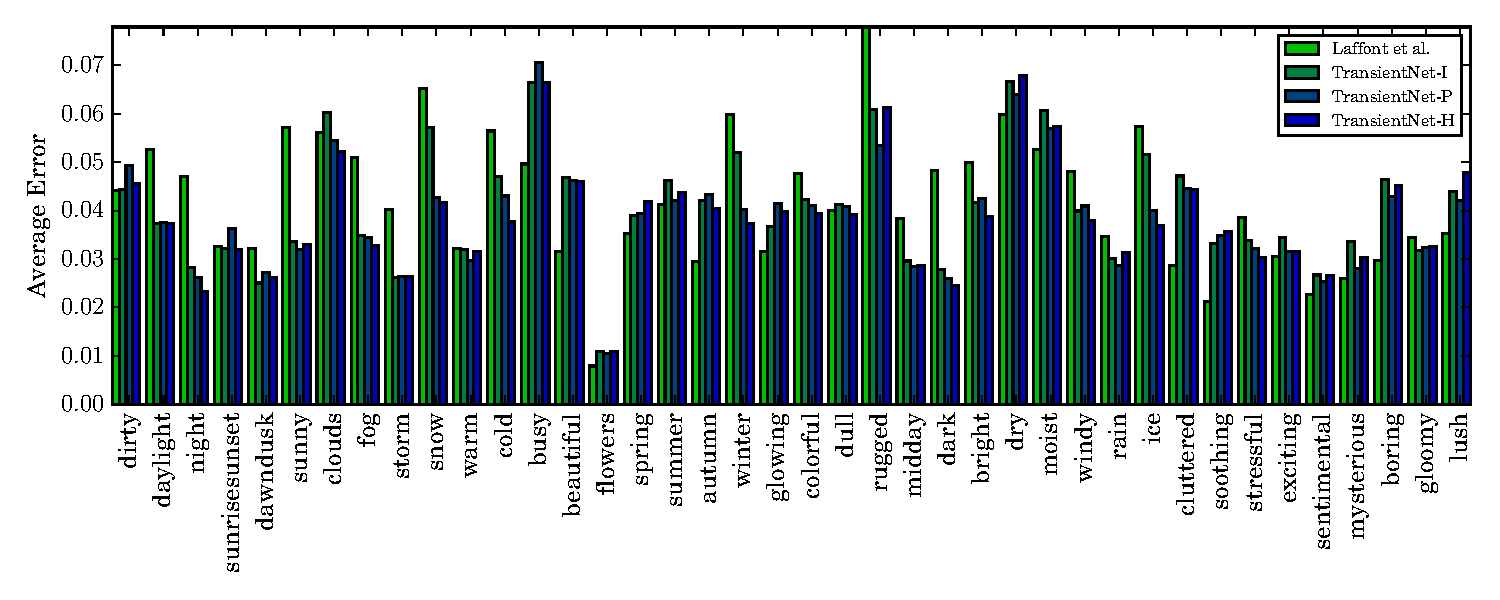
\includegraphics[width=1.0\textwidth, trim= 0 4mm 0 0]{figs/avg_err_compare.pdf}
%		\caption{This shows the average errors for each attribute from the method proposed
%						 by Laffont et al., and our three networks: TransientNet-I, TransientNet-P,
%             and TransientNet-H.  TransientNet-H has the lowest average error for a 
%             majority of the attributes.}
%		\label{fig:compare}
%\end{figure*}

\vspace{-1em}
\paragraph{CloudyNet:} For the problem of classifying whether an image is sunny or
cloudy, we use the data provided by Lu et al.~\cite{lutwoclass} to train our
network, which we call CloudyNet. 
The dataset contains $10\,000$ images collected from the SUN
Database~\cite{xiaoSUN}, the LabelMe Database~\cite{russell2008labelme}, and
Flickr. Each image is assigned a ground-truth binary label,
sunny or cloudy, by a human rater.
% nbj: probably don't need to say this here\dots and this isn't really
% five-fold cross validation since you are rerandomizing between
% splits
%During evaluation we report the mean and variance
%of normalized accuracy using five-fold cross validation. 
We convert \emph{AlexNet} into CloudyNet by modifying the network
architecture; we 
drop the final fully connected layer and replace it with a
fully connected layer with two output nodes.

\vspace{-1em}
\paragraph{TransientNet:} For the more challenging problem of estimating the
presence of a broad range of attributes in an image, we use the dataset
introduced by Laffont et al.~\cite{Laffont14}.  The dataset contains images
from outdoor webcams in the Archive of Many Outdoor Scenes~\cite{jacobs07amos}
and the Webcam Clip Art Dataset~\cite{lalondesig09}.  The webcams span a wide
range of outdoor scenes, from urban regions to wooded, mountainous regions.
Each webcam has 60--120 images captured in a wide range of conditions at
different times of day and on different days of the year.  The final dataset
consists of $8\,571$ high resolution images from 101 webcams.  The authors
define a set of 40 transient attributes, each of which is assigned a value
between zero and one, representing the confidence of that attribute appearing
in an image. We modify the \emph{AlexNet} network architecture by changing the final
fully connected layer to have 40 output nodes, one for each transient
attribute, and updating the loss function to an $L_2$ loss. We call the
resulting network TransientNet. 

\vspace{-1em}
\paragraph{Network Training:} For each network architecture, we start the training procedure from three different initial conditions,
resulting in six distinct sets of network weights. The first set of initial
conditions were taken from a network that was was trained for object
classification on 1.2 million images from the ImageNet ILSVRC-2012
challenge~\cite{ILSVRCarxiv14}.  We call the networks that result from this
fine-tuning process CloudyNet-I and TransientNet-I.  The second set of initial
conditions were taken from a network~\cite{zhou2014places} that was trained for
scene classification on 2.5 million images with labels in 205 categories from
the Places Database~\cite{zhou2014places}. We call the resulting networks
CloudyNet-P and TransientNet-P.  The final set of initial conditions were taken
from a network~\cite{zhou2014places} that was trained for both object and scene
classification.  This hybrid network was trained on a combination of the Places
Database~\cite{zhou2014places} and images from the training data of ILSVRC-2012
challenge~\cite{ILSVRCarxiv14}.  The full training set contained 205 scene
categories from the Places Database and 978 object categories from ILSVRC-2012
containing about 3.6 million images.  We call the resulting networks CloudyNet-H
and TransientNet-H.

%\textbf{Expanded Dataset:} We expand the Transient Attributes dataset from
%Laffont et al.~\cite{Laffont14} using AMOS~\cite{jacobs07amos} webcams.  We
%first find the geolocation of the AMOS webcams within the transient attributes
%dataset.  Images from cameras with locations near these webcams are downloaded.
%Images from nearby webcams with corresponding timestamps to images in the
%Transient Attributes Dataset are assigned the ground truth labels from the
%dataset.  This is based on the idea that nearby webcams should have similar
%transient attributes at any given time. 
%\todo{get more specifics from Ted} 
%
%\textbf{Partial Siamese TransientNet:}

\vspace{-1em}
\paragraph{Implementation Details:} Our networks are trained using the
Caffe~\cite{caffe14} deep learning framework, the CaffeNet reference network
architecture (a variant of \emph{AlexNet}), and pre-trained networks from the
Caffe Model Zoo~\cite{modelzoosite}.  The full network optimization definition,
the final network weights, and the output from our methods are available on the
project webpage (\url{http://cs.uky.edu/~rbalten/transient}).

%All of our networks were trained on NVIDIA M2075 GPU Cards for 24
%hours each, and evaluated using Caffe in CPU mode on Dell C6220
%Servers equipped with Dual Intel E5-2670 8 Core (Sandy Bridge)
%processors at 2.6 GHz.  

\begin{table}[t]
	\centering
	\caption{Two class weather classification accuracy}
	\begin{tabular}{ | l | c | }
		\hline
			Method & Normalized Accuracy \\ \hline \hline
			Lu et al.~\cite{lutwoclass}& $ 53.1 \pm 2.2 $ \\ \hline
			CloudyNet-I & $ 85.7 \pm 0.5 $ \\ \hline
			CloudyNet-P & $ 86.1 \pm 0.6 $ \\ \hline
			CloudyNet-H & $ \textbf{87.1} \pm 0.3 $ \\ 
		\hline
	\end{tabular}
	\label{tbl:twoclass}
\end{table}

\begin{table}[t]
	\centering
	\caption{Transient attribute prediction errors}
	\begin{tabular}{ | l | c | }
		\hline
			Method & Average Error \\ \hline \hline
			Laffont et al.~\cite{Laffont14}& 4.2\% \\ \hline
			TransientNet-I & 4.05\% \\ \hline
			TransientNet-P & 3.87\% \\ \hline
			TransientNet-H & \textbf{3.83\%} \\ 
		\hline
	\end{tabular}
	\label{tbl:transient}
\end{table}

\section{Evaluation}

We evaluated our networks on two benchmark datasets. The results show
that our proposed approaches are significantly faster and more
accurate than previous methods. 

\subsection{Two-Class Weather Classification}

We evaluated our three CloudyNet variants using the dataset created by Lu et
al.~\cite{lutwoclass} (introduced in Section~\ref{sec:method}). 
We follow their protocol for
generating a train/test split: we randomly shuffle sunny/cloudy images
and then select 80\% of each class for training and 20\% for testing.
This process is repeated five times resulting in five random 80/20
splits of the data. 
%Flickr images
%were collected manually by ``helpers'' unaware of the purpose or methods of Lu
%et al. The dataset was then pruned for images with similar histograms, and
%finally pruned by another round of helpers to narrow the dataset to 10,000
%images.
\tblref{twoclass} shows the mean normalized accuracy and variance for our
networks and the previous best technique.  The normalized accuracy, which is
the proposed evaluation metric by Lu et al., is calculated by $ \max\{((a -
0.5) / 0.5), 0\} $, where $a$ is the traditionally obtained accuracy. All three
of our networks outperform the state of the art for two class weather
classification with CloudyNet-H predicting the most accurately.

%Our method is also very fast; it averages 0.0672s per
%image for prediction. 

\subsection{Transient Attributes Estimation}

We evaluated our three TransientNet variants on the dataset created by Laffont
et al.~\cite{Laffont14}.  We use the same holdout train/test split in which
images from 81 webcams are used for training and images from a distinct set of
20 other webcams are used for testing. 
%TransientNet-H performs best on more than half of the attributes and is the
%best performing CNN that we trained.
TransientNet-H has the lowest overall average error as shown in
\tblref{transient}.  TransientNet-P and TransientNet-H have similar
performance, mostly due to them being pre-trained on similar sets of data.

%\tblref{timing} compares the average prediction speed for the method provided
%by Laffont et al.~\cite{Laffont14} and our best performing network,
%TransientNet-H. 

In addition to having higher accuracy, our method is significantly faster.  For
a single image, Laffont et al.'s method takes an average of 3.486 seconds, but
our method only requires 0.192 seconds, an 18x speed up. 

\begin{figure}[t]
	\centering
		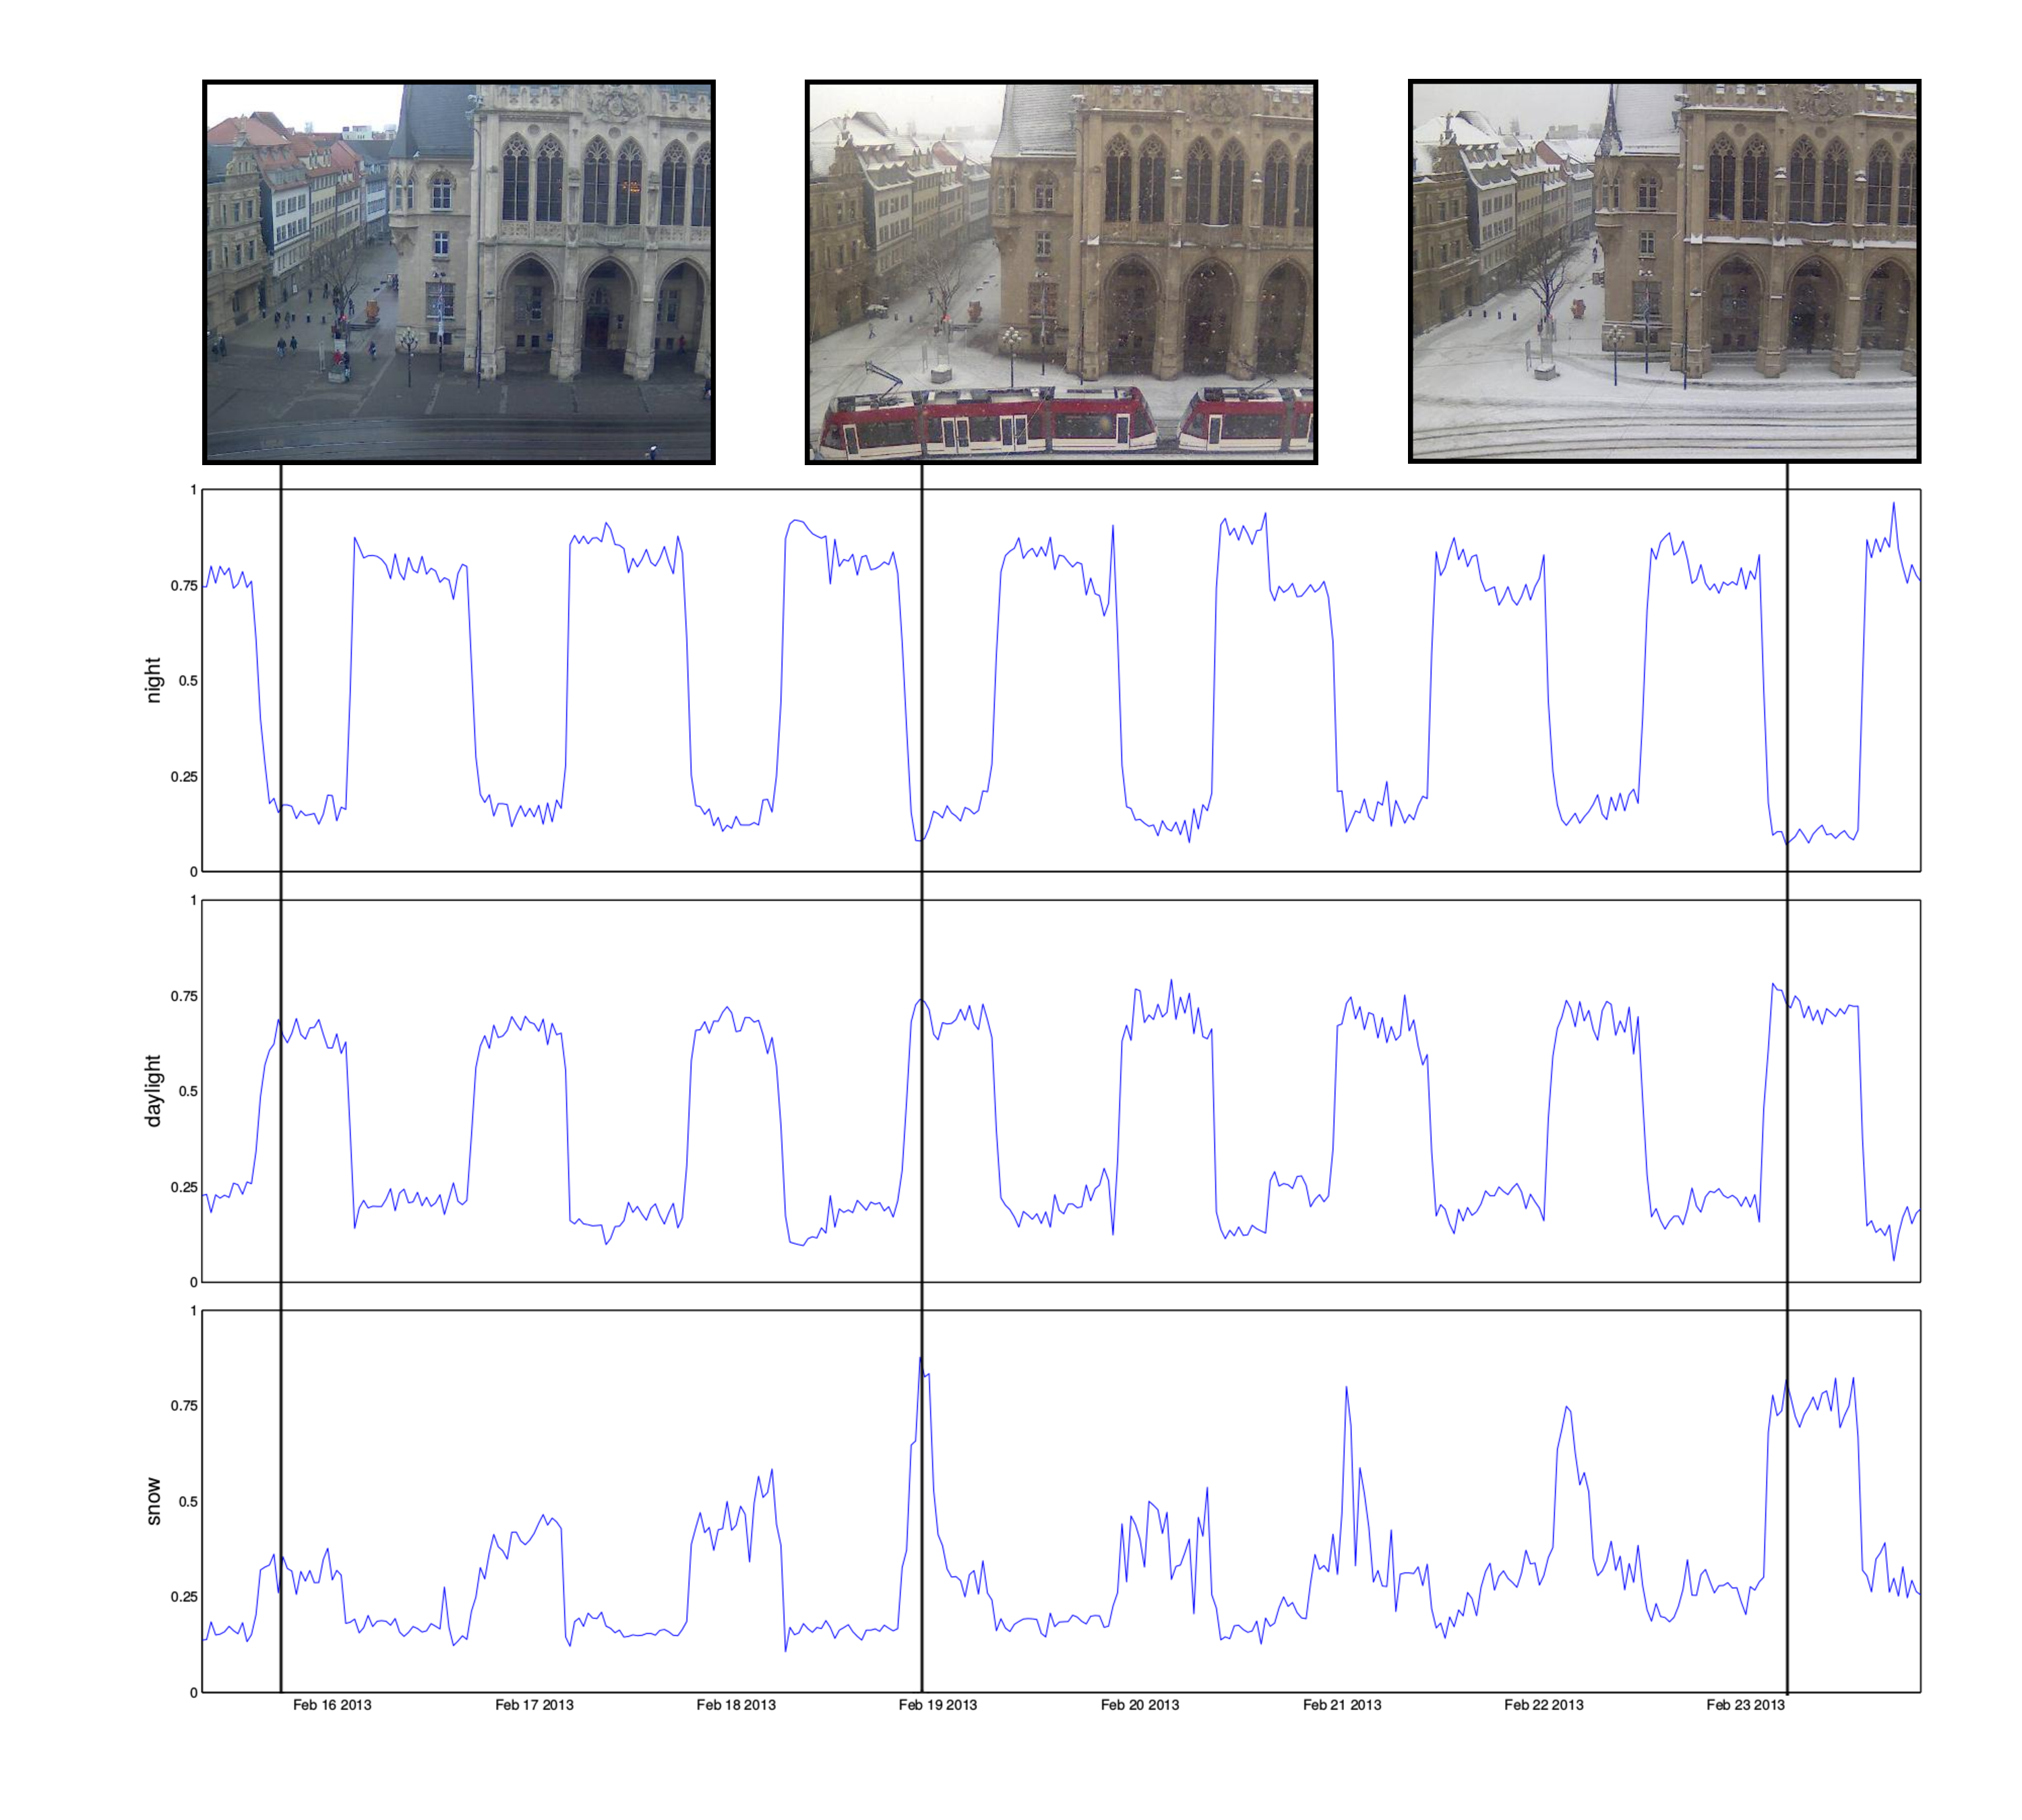
\includegraphics[width=\linewidth, trim= 5mm 15mm 0mm 10mm]{figs/attr_compare.pdf}
		\caption{A snapshot of three attributes over a week of webcam data.
             The highlighted images show the scene at the given point in time.}
		\label{fig:attrcmp}
\end{figure}

\subsection{Example Results}

\begin{figure}[t]
	\centering
		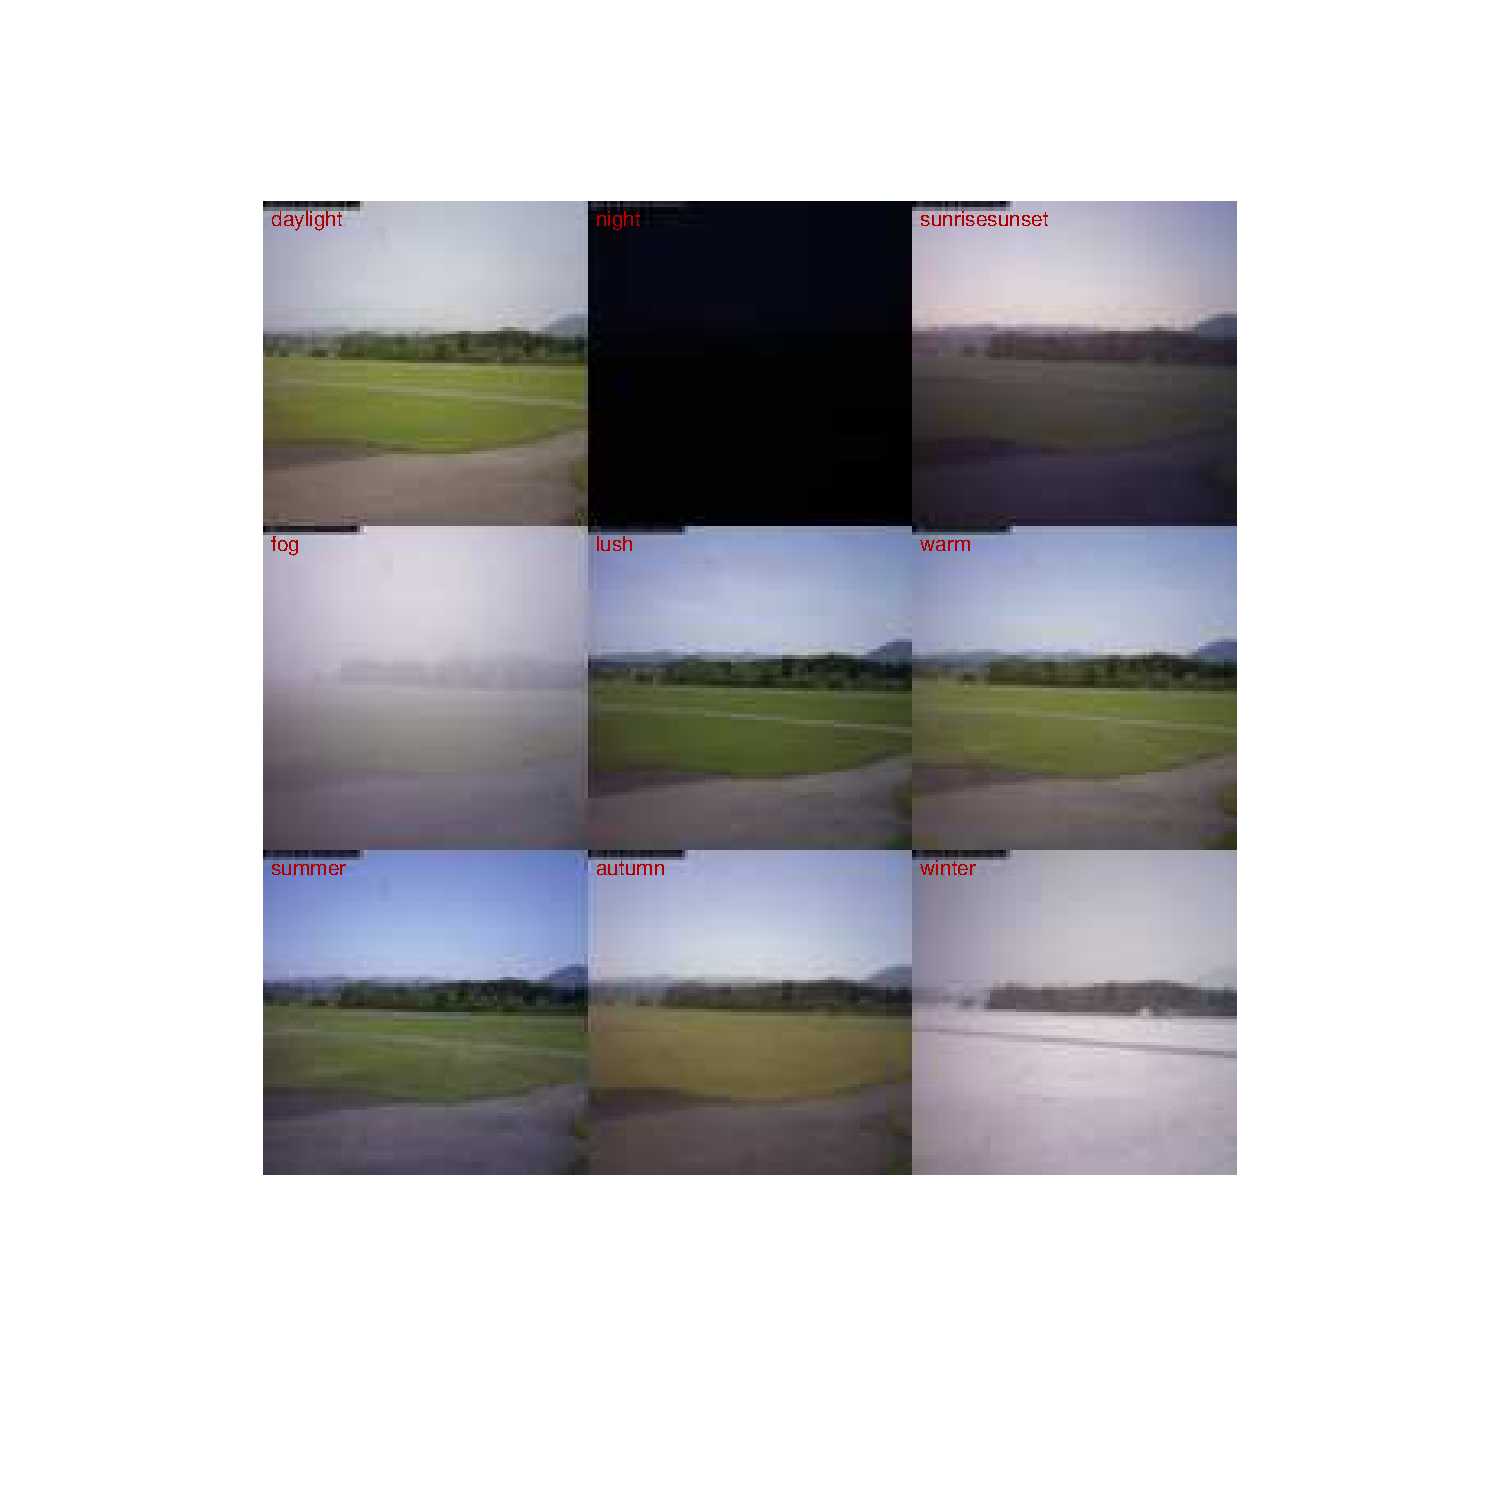
\includegraphics[width=\linewidth]{figs/montage_pruned_cam_7211.pdf}
		\caption{The average of the 100 most confident images for
             a subset of transient attributes from a given webcam.} 
		\label{fig:netvis}
\end{figure}

%We look at the values for selected attributes over a given span of time and
%their corresponding webcam images.  We qualitatively confirm the predicted
%attribute values and visualize the scene which maximizes each attribute.

As qualitative evaluation, \figref{attrcmp} shows the time series
of the predicted value (using TransientNet-H) for three attributes
(\textit{night, daylight, and snow}) from an AMOS~\cite{jacobs07amos}
webcam over the period February 16th, 2013 to February 23rd, 2013.
Note that no temporal smoothing was performed, these are raw per-image
estimates.  The inverse relationship between the \textit{daylight} and
\textit{night} time series can be clearly seen.  \figref{attrcmp} also
shows images of the scene captured at different times, highlighting
snowy and non-snowy periods.

\figref{netvis} shows semantic average images for a single scene.  Each
image is the average of the 100 images with the highest score for a particular
attribute.  The subset of attributes shown in \figref{netvis} represent a wide
variety of conditions of the scene.  The seasonal attributes (\textit{autumn,
summer, winter}) show how the scene changes throughout the year and lighting
attributes (\textit{sunrise/sunset, daylight, night}) shows the scene in
various lighting conditions.  Such images are easy to create and highlight the
ability of our proposed technique to work across a broad range of conditions
and scene types. 

\figref{ex_bad_transientnet} shows examples of images with an attribute that
TransientNet-H mislabeled.  \figref{ex_bad_snow} shows a white-sand beach that
was labeled as being a snowy image.  \figref{ex_bad_daylight} shows a lit
sports arena at night that was labeled as being a daylight image.
\figref{ex_bad_cloudynet} shows examples of misclassified images using
CloudyNet-H.  \figref{ex_bad_cloudy} shows an outdoor arch that was
misclassified as sunny.  \figref{ex_bad_sunny} shows a uniformly lit outdoor
garden that was misclassified as cloudy.

%Other attributes not shown in this montage have similar average
%images to the ones shown, (\textit{e.g., glowing and colorful similar to
%sunrise/sunset, windy and rain similar to fog}).  This suggests that the
%network may not distinguish between these attributes well or that these
%attributes have some correlation with each other.

%Labeling a million images using
%Laffont et al.'s method on a single machine would take upwards of 40
%days, whereas our network on a single machine would take approximately
%2.2 days.  

%\todo{edit this text to not talk about rel err plot}
%
%\figref{relerr} shows the relative error between our method using
%TransientNet-H and the method presented by Laffont et al.~\cite{Laffont14}  The
%average relative error for each attribute using the method by Laffont et al.\
%was subtracted from the average relative error using TransientNet-H.  A
%negative value means TransientNet-H had a smaller error and a positive value
%means Laffont et al. had a smaller error.  For example, the difference between
%the two methods on the attribute \emph{night} was around 2.5 percentage points,
%with TransientNet-H having the smaller error.  TransientNet-H averages 0.0699s
%per image for prediction. 

%\begin{table}[t]
%	\centering
%	\caption{Transient attribute prediction speed}
%  \begin{tabular}{ | l | p{.35\linewidth} | }
%		\hline
%			Method & Prediction Time (avg. per image) \\ \hline \hline
%			Laffont et al.~\cite{Laffont14}& $ 3.486 s $ \\ \hline
%			TransientNet-H & $ \textbf{0.192 s} $ \\ 
%		\hline
%	\end{tabular}
%	\label{tbl:timing}
%\end{table}

%\begin{figure}[t!]
%  \renewcommand{\arraystretch}{1.6}
%  \centering
%  \begin{tabular}[b]{| c | c |}
%    \hline
%    Image & Labels \\
%    \hline \hline
%    \multirow{3}[3]{*}[-2mm]{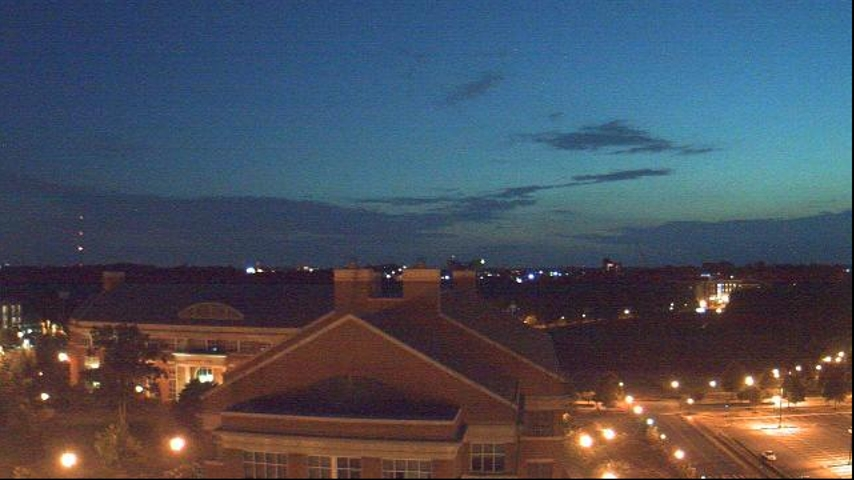
\includegraphics[width=0.19\textwidth]{figs/labels_1.jpg}}
%      & night, not sunny \bigstrut \\
%      & dark, not snow \bigstrut  \\
%      & glowing, not midday \bigstrut  \\
%    \hline
%    \multirow{3}[3]{*}[-1mm]{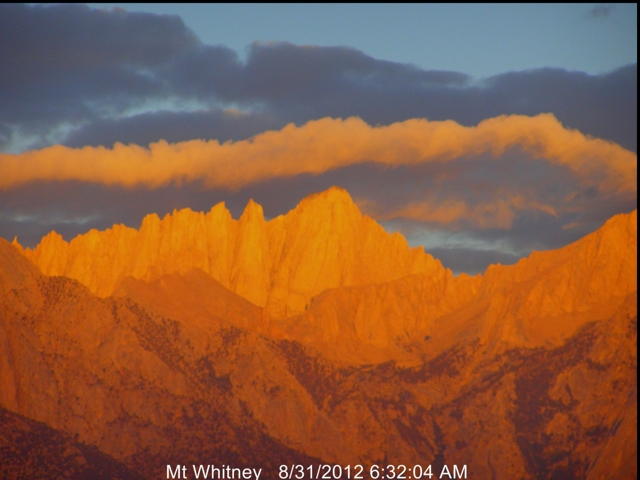
\includegraphics[width=0.17\textwidth]{figs/labels_2.jpg}}
%      & rugged, not flowers \bigstrut  \\
%      & dawndusk, not rain \bigstrut  \\
%      & sunrisesunset, not storm  \bigstrut \\
%    \hline
%  \end{tabular}
%  \caption{Example labels for images using TransientNet-H}
%  \label{fig:labels}
%\end{figure}

% I think we could do without this plot as well.  At the very least
% we should get rid of this plot or the bigger bar chart
%\begin{figure}[t!]
%	\centering
%		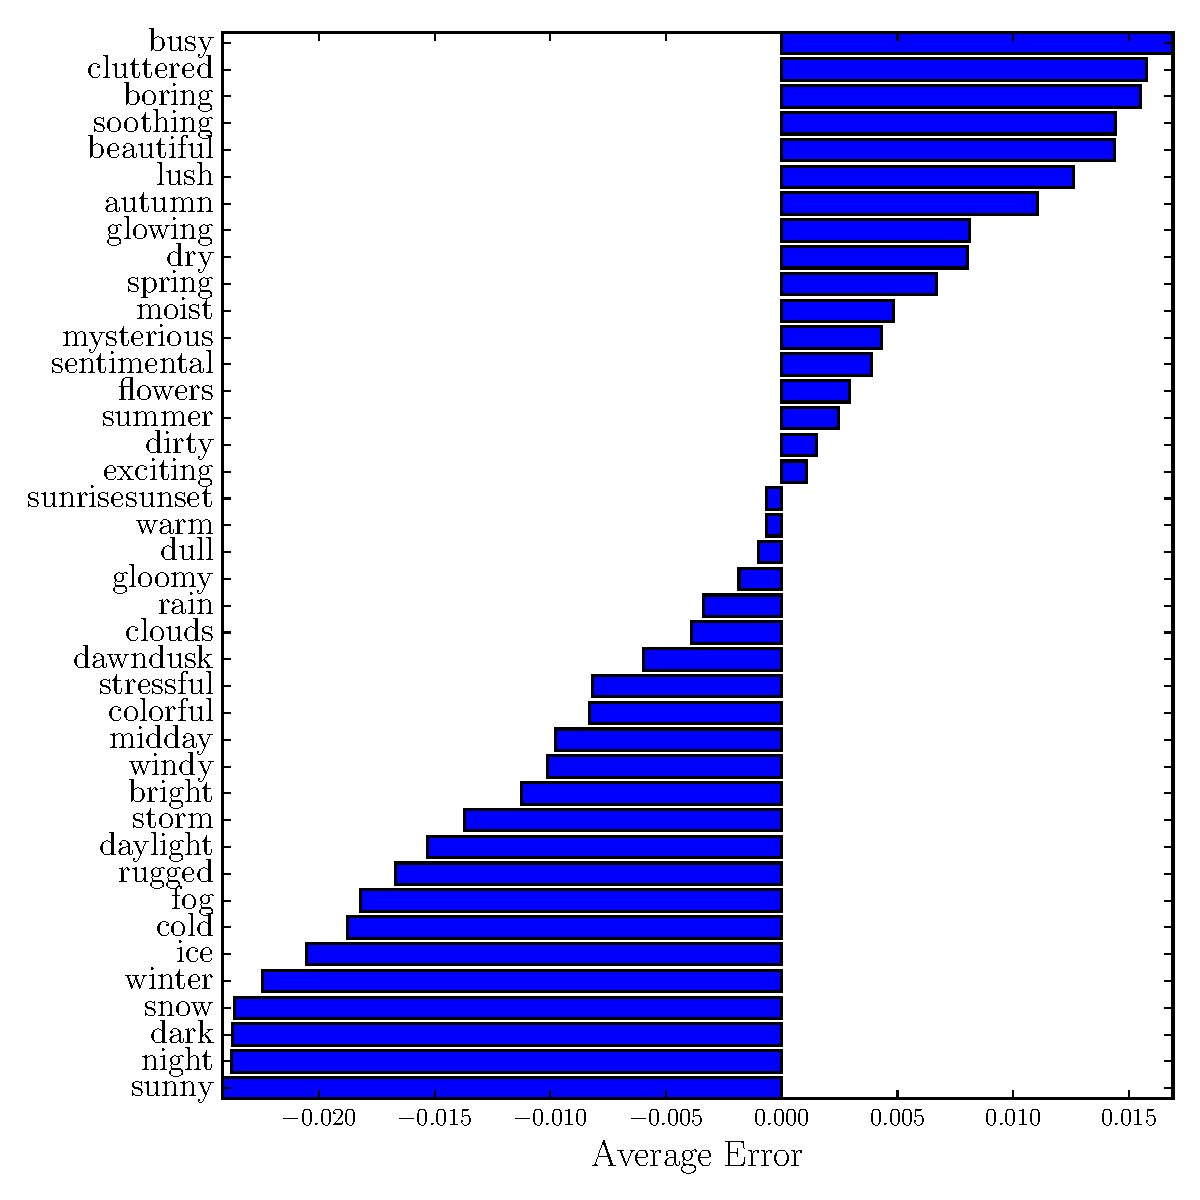
\includegraphics[width=0.5\textwidth]{figs/rel_err_cmr.pdf}
%		\caption{This shows the relative errors of TransientNet-H against the method 
%						 proposed by Laffont et al. for each attribute.  Attributes with a 
%						 negative average error are attributes that are predicted more 
%						 accurately by our method.}
%		\label{fig:relerr}
%\end{figure}


\begin{figure*}
  \centering
  \begin{subfigure}[b]{0.46\textwidth}
    \centering
		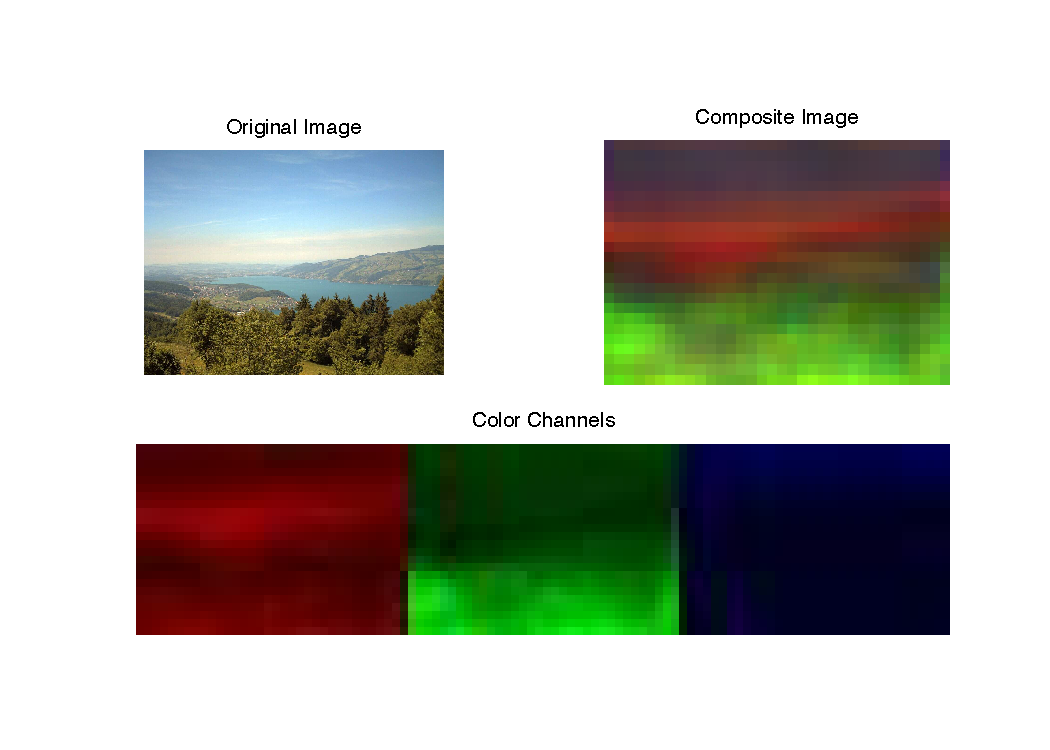
\includegraphics[width=\textwidth]{figs/false_color_7371.pdf}
    \caption{RGB = [\textit{sunny, lush, snow}]}
    \label{fig:false_color_1}
  \end{subfigure}
  \hfill
  \begin{subfigure}[b]{0.46\textwidth}
    \centering
		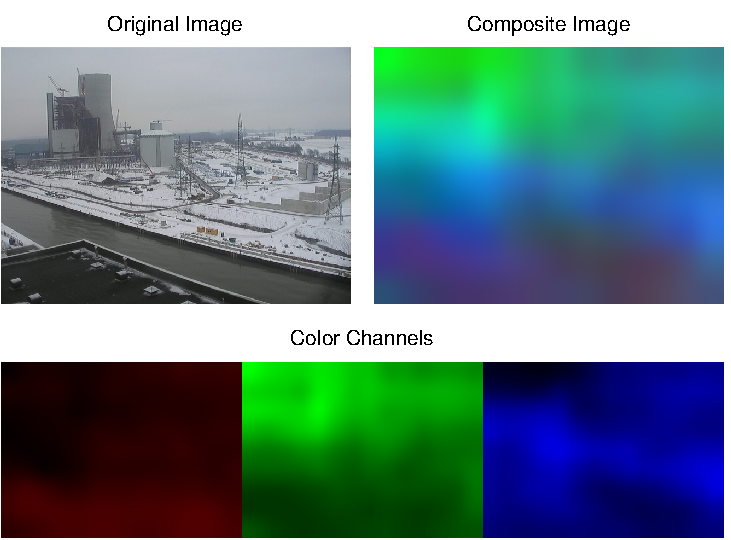
\includegraphics[width=\textwidth]{figs/false_color_82.pdf}
    \caption{RGB = [\textit{sunny, storm, snow}]}
    \label{fig:false_color_2}
  \end{subfigure}
  \caption{Composite images generated using the fully convolutional TransientNet-H.
           Brighter areas in each of the color channels indicate a high
           attribute value.}
  \label{fig:false_color_ims}
\end{figure*}

\begin{figure}
	\centering
  \begin{subfigure}[b]{\columnwidth}
    \centering
		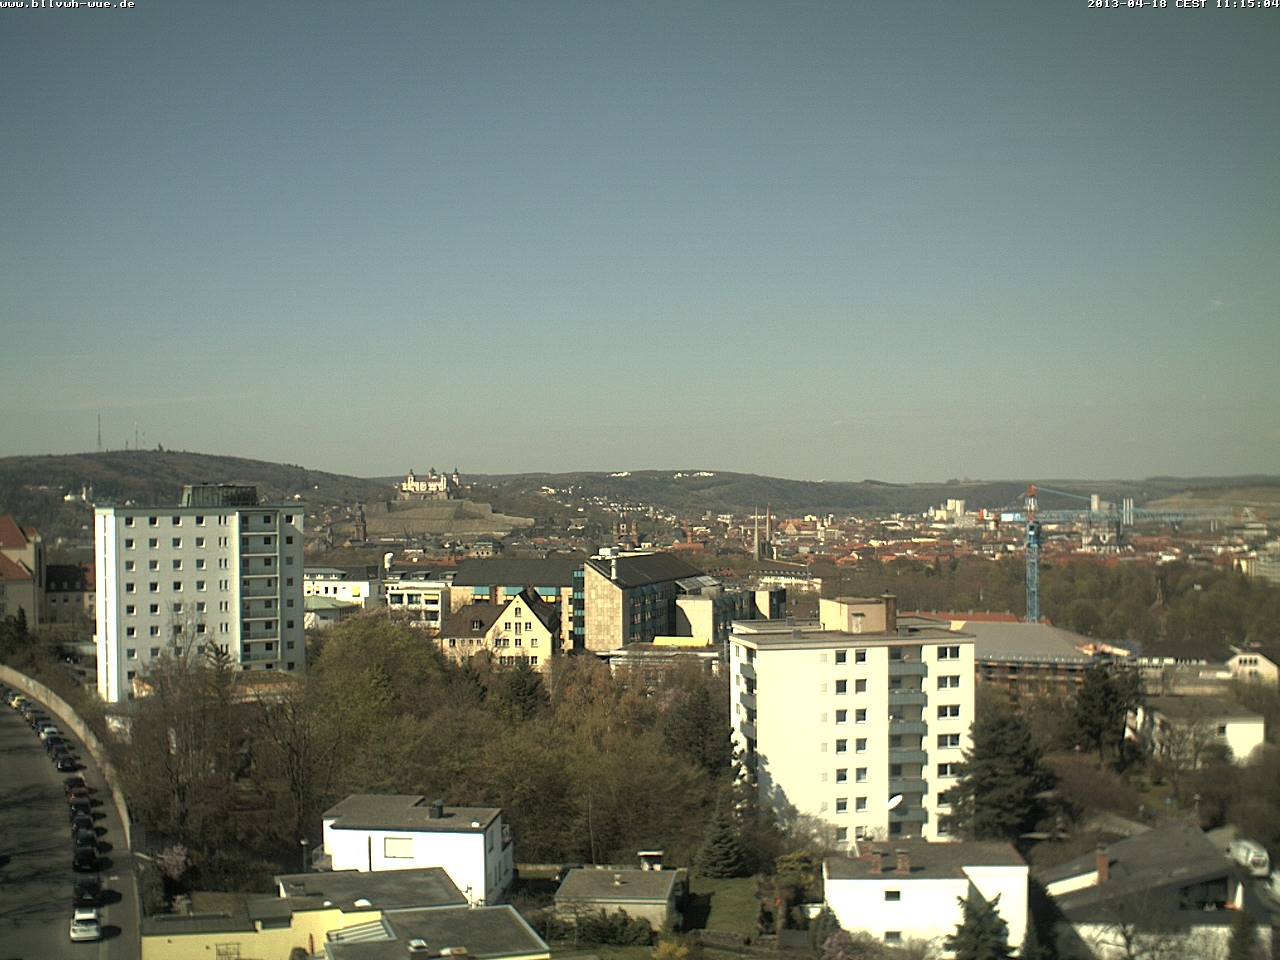
\includegraphics[width=0.49\columnwidth]{figs/cam_summary/3396_04180908.jpg}
		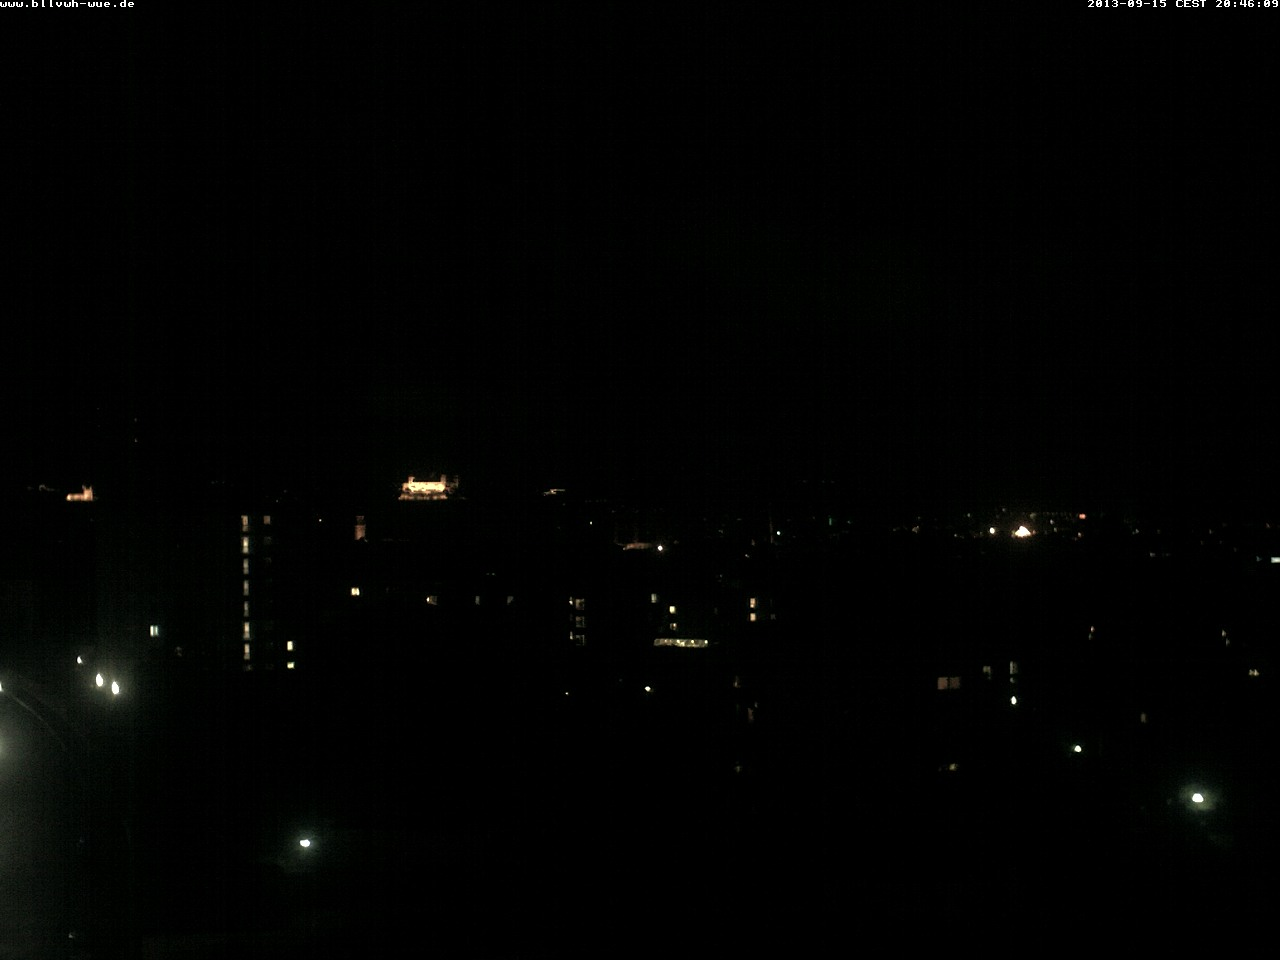
\includegraphics[width=0.49\columnwidth]{figs/cam_summary/3396_09151838.jpg}
		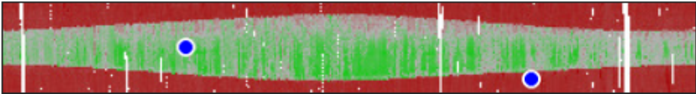
\includegraphics[width=\columnwidth]{figs/cam_summary/00003396_daylight.pdf}
    \caption{\emph{Daylight}}
    \label{fig:daylight}
	\end{subfigure}	
  \begin{subfigure}[b]{\columnwidth}
    \centering
		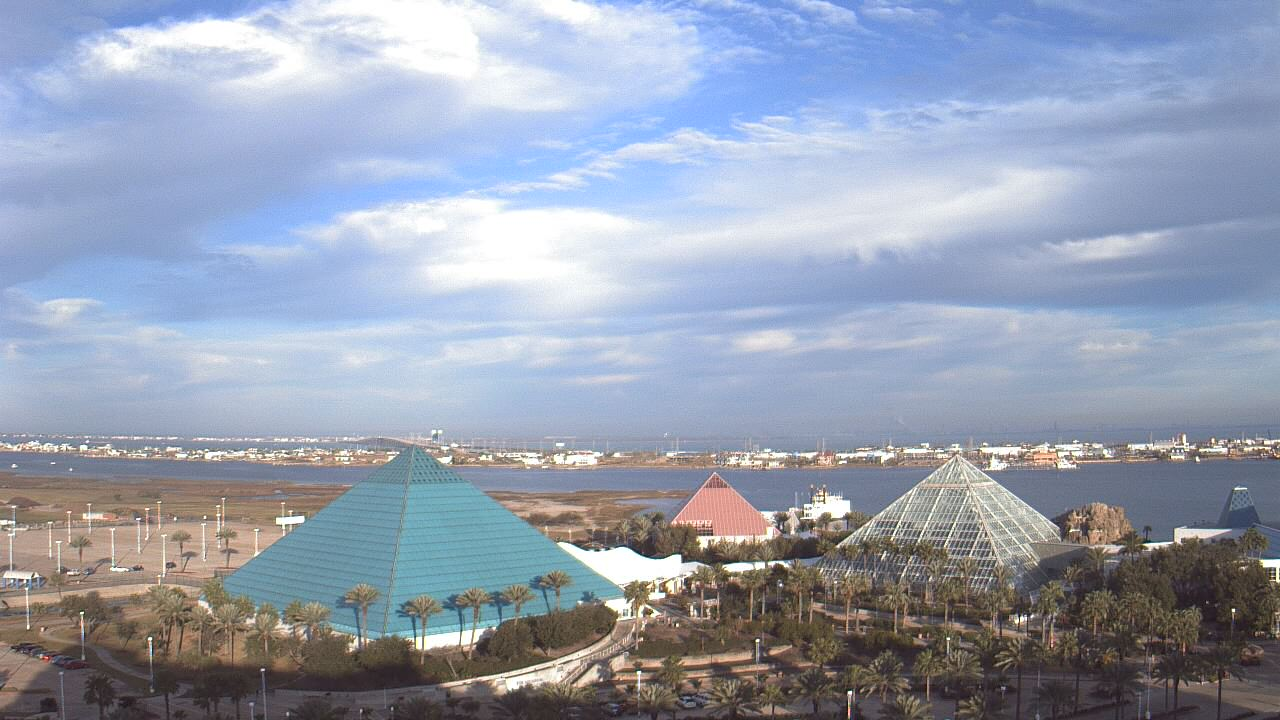
\includegraphics[width=0.49\columnwidth]{figs/cam_summary/623_01191411.jpg}
		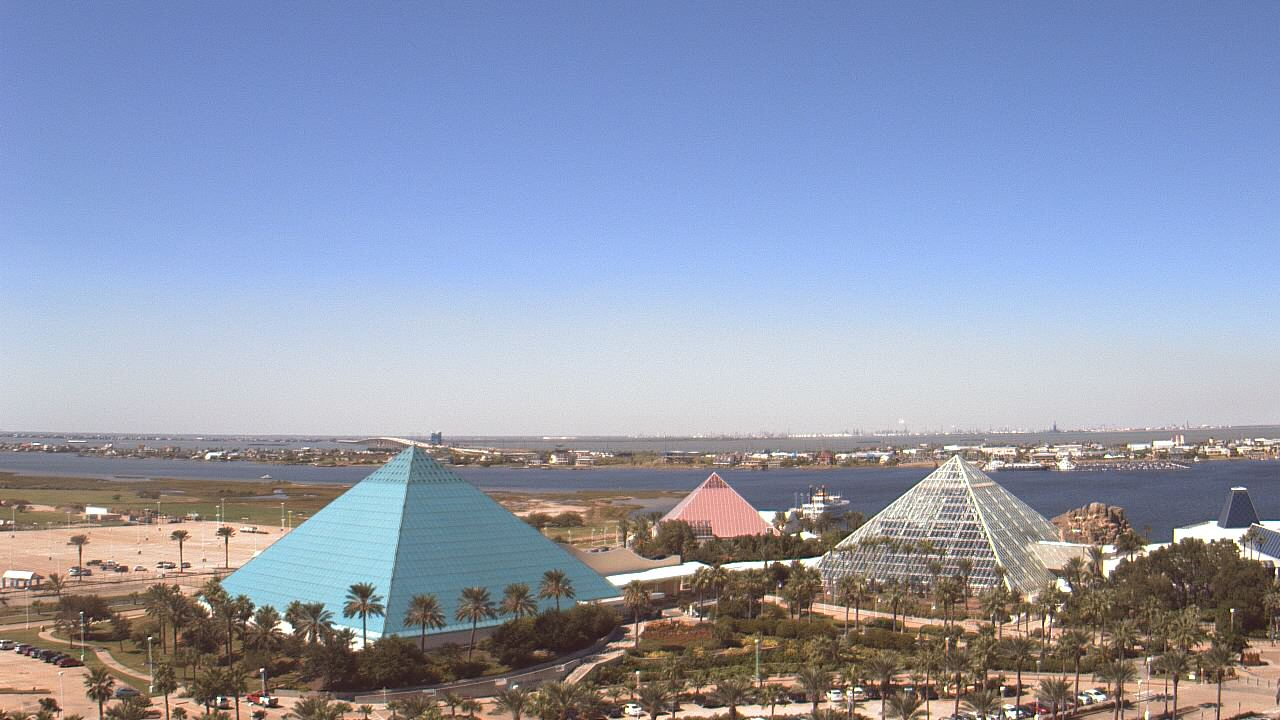
\includegraphics[width=0.49\columnwidth]{figs/cam_summary/623_10071911.jpg}
		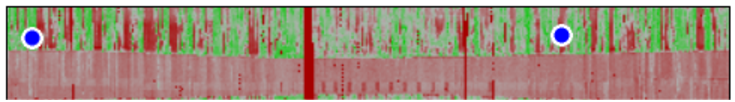
\includegraphics[width=\columnwidth]{figs/cam_summary/00000623_clouds.pdf}
    \caption{\emph{Clouds}}
    \label{fig:clouds}
	\end{subfigure}	
  \begin{subfigure}[b]{\columnwidth}
    \centering
		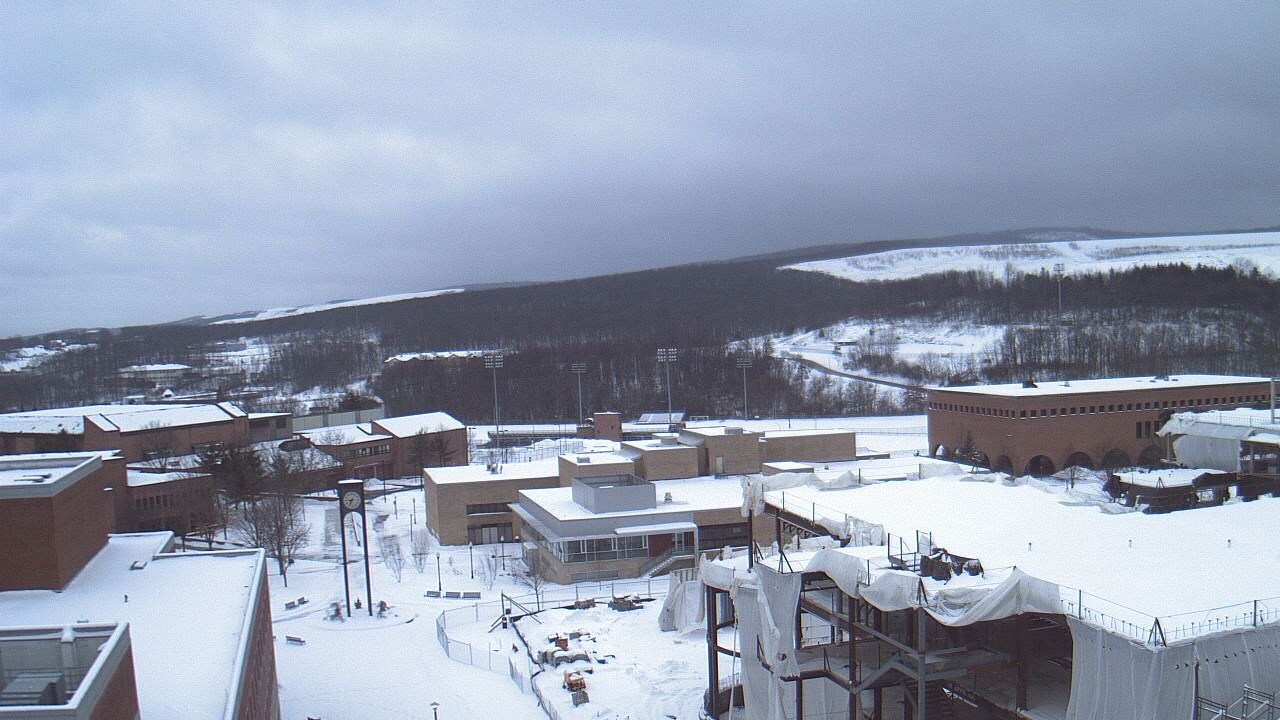
\includegraphics[width=0.49\columnwidth]{figs/cam_summary/260_01011844.jpg}
		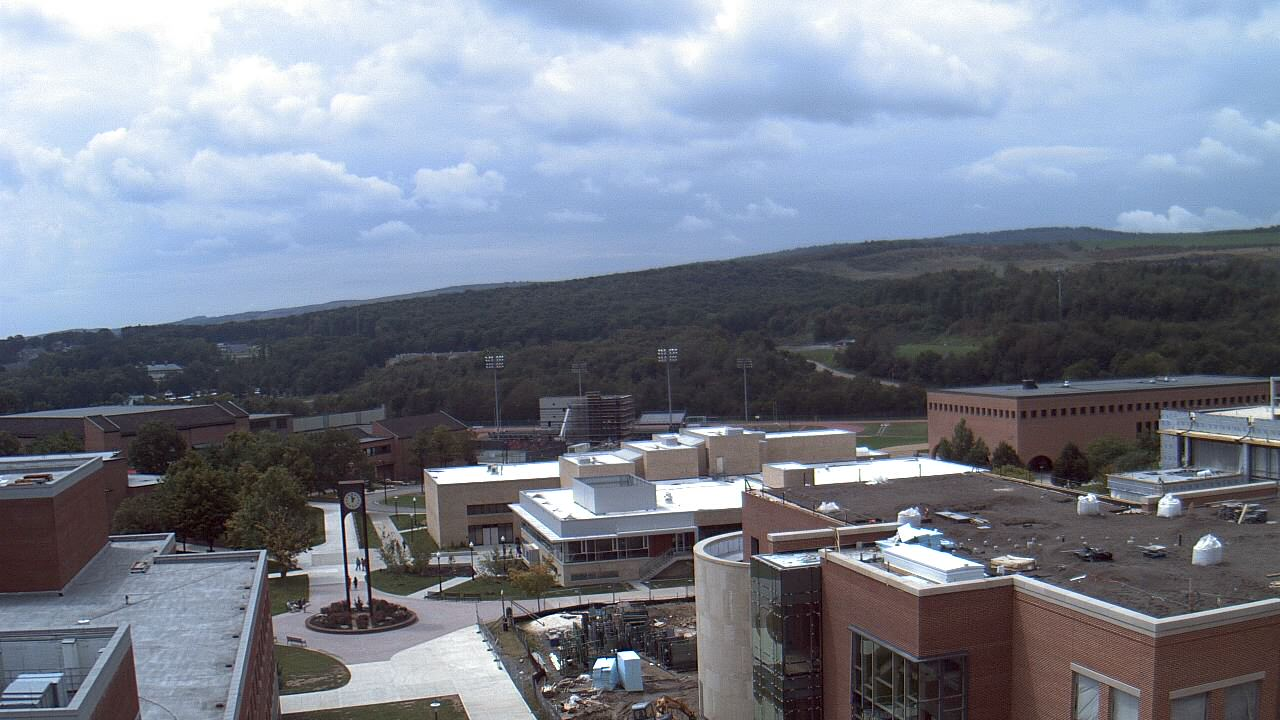
\includegraphics[width=0.49\columnwidth]{figs/cam_summary/260_09011714.jpg}
    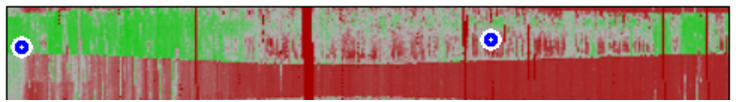
\includegraphics[width=\columnwidth]{figs/cam_summary/00000260_snow.pdf}
    \caption{\emph{Snow}}
    \label{fig:snow}
	\end{subfigure}	
	\caption{Example attribute summaries over a year of webcam data.  The highlighted
           images are denoted by the blue dots within each attribute summary.}
	\label{fig:webcam_summary}
\end{figure}

%\begin{figure}[t]
%	\centering
%		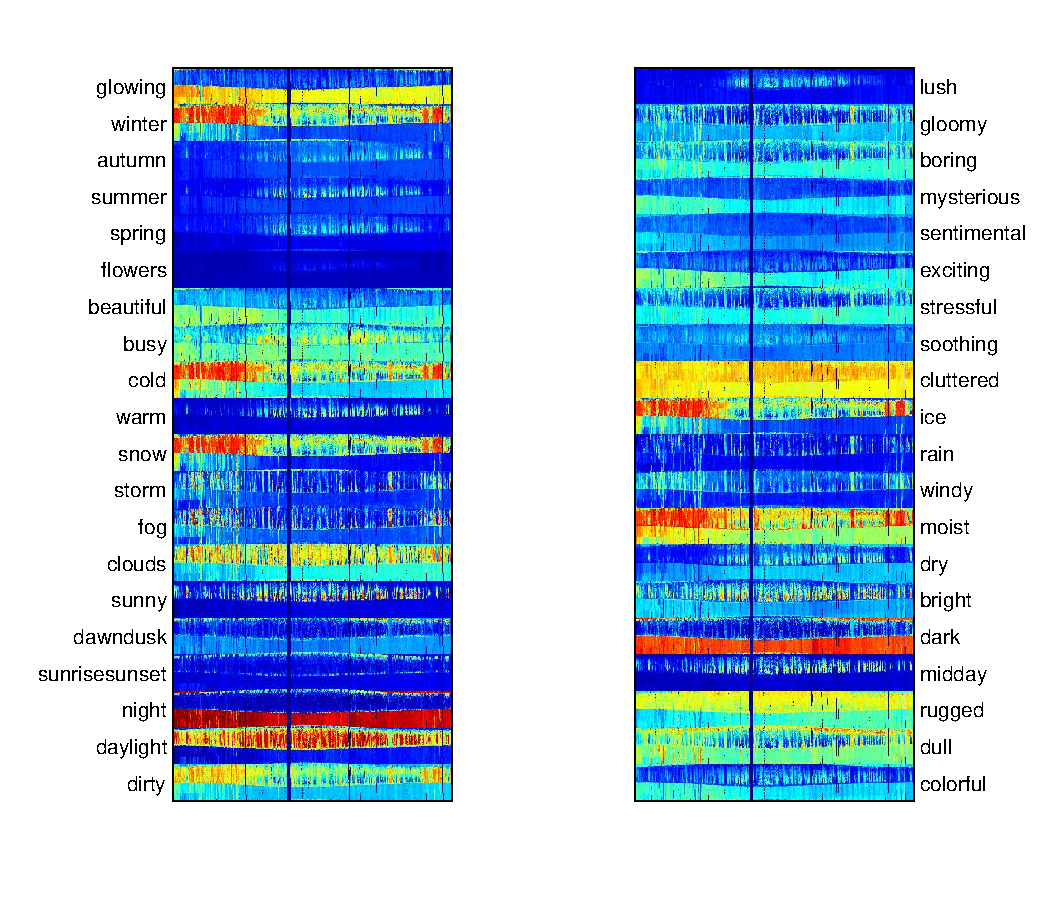
\includegraphics[width=0.5\textwidth, trim= 5mm 15mm 0mm 10mm]{figs/summary_260.pdf}
%		\caption{The transient attribute values for a year of webcam 
%             data.  Each column corresponds to a day of the year and each row
%             corresponds to a time of day.}
%		\label{fig:webcam_summary}
%\end{figure}


\subsection{Rapidly Labeling Sub-Images}

\begin{figure}
	\centering
  \begin{subfigure}[b]{0.49\columnwidth}
    \centering
		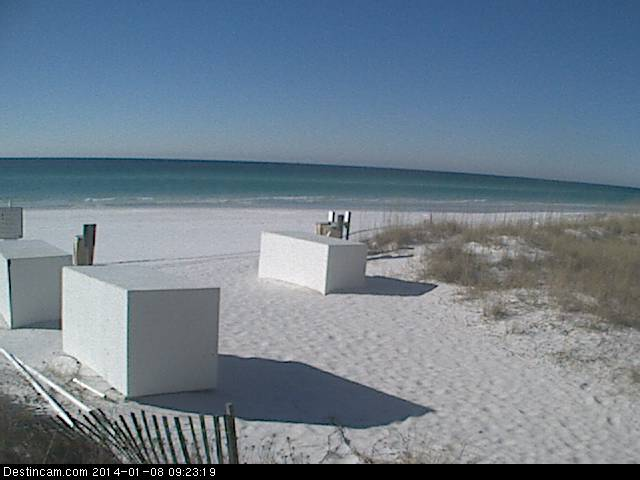
\includegraphics[width=\columnwidth]{figs/ex_bad_ims/snow_bad_1.jpg}
    \caption{Mislabeled \emph{snow}}
    \label{fig:ex_bad_snow}
	\end{subfigure}	
  \begin{subfigure}[b]{0.49\columnwidth}
    \centering
		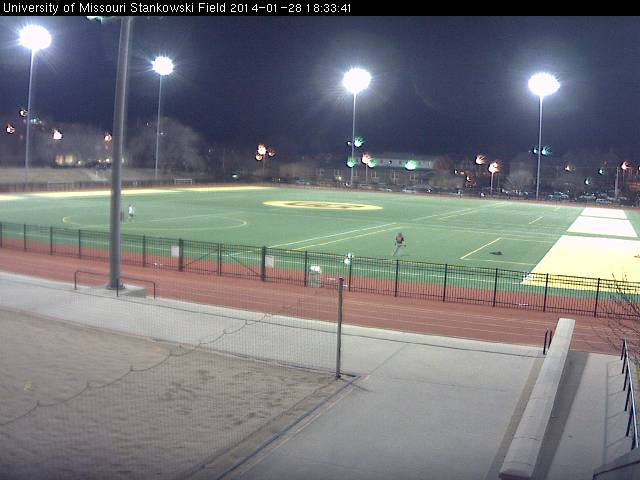
\includegraphics[width=\columnwidth]{figs/ex_bad_ims/daylight_bad_1.jpg}
    \caption{Mislabeled \emph{daylight}}
    \label{fig:ex_bad_daylight}
	\end{subfigure}	
	\caption{Two failure cases using TransientNet and their mislabeled attribute.}
	\label{fig:ex_bad_transientnet}
\end{figure}

\begin{figure}
	\centering
  \begin{subfigure}[b]{0.49\columnwidth}
    \centering
		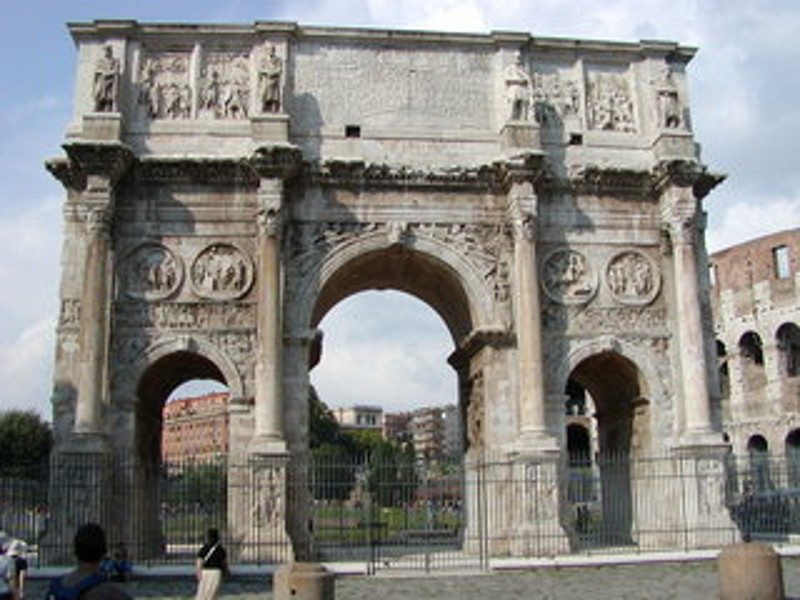
\includegraphics[width=\columnwidth]{figs/ex_bad_tc/cloudy_3732.jpg}
    \caption{Misclassified \emph{sunny}}
    \label{fig:ex_bad_cloudy}
	\end{subfigure}	
  \begin{subfigure}[b]{0.49\columnwidth}
    \centering
		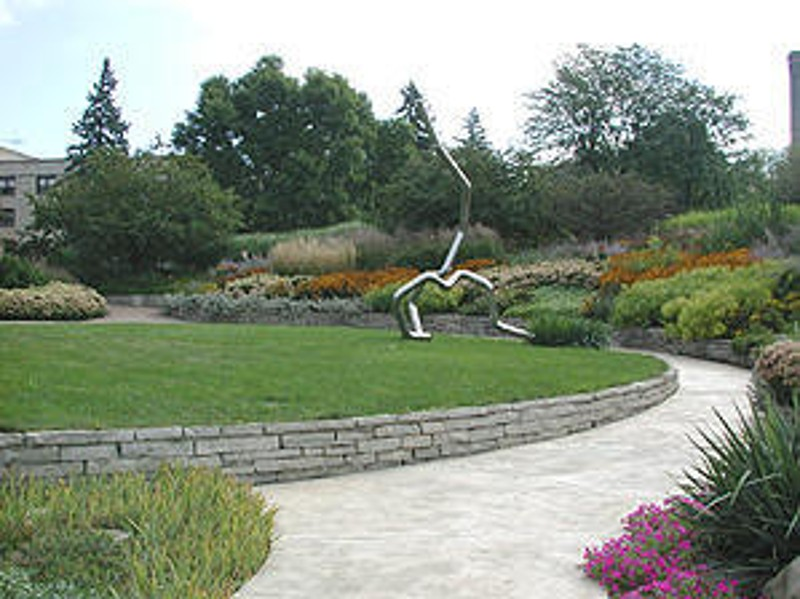
\includegraphics[width=\columnwidth]{figs/ex_bad_tc/sunny_2877.jpg}
    \caption{Misclassified \emph{cloudy}}
    \label{fig:ex_bad_sunny}
	\end{subfigure}	
	\caption{Two failure cases using CloudyNet and their misclassified class.}
	\label{fig:ex_bad_cloudynet}
\end{figure}

We convert the final, fully connected layers of TransientNet to be
convolutional~\cite{long2015fully} with the same number of outputs.  The output
from this new, ``fully convolutional'' network allows us to create images
showing an attribute's value across an input image, as shown in
\figref{false_color_ims}.  The values for each attribute can be visualized in a
single channel image.  Combining three of these images results in the composite
images.  \figref{false_color_1} shows a composite image using the
\textit{sunny}, \textit{lush}, and \textit{snow} attributes as the color
channels.  As expected, there are no snowy areas in the input image, shown in
the blue channel, and the bottom of the image contains high values for the lush
attribute, shown in the green channel.  The sunny attribute is higher towards
the horizon and middle of the sky, show in the red channel, possibly due to the
sky being brighter in these regions.  \figref{false_color_2} shows a composite
image using the \textit{sunny}, \textit{storm}, and \textit{snow} attributes as
the color channels.  The image has low values for the sunny attribute, shown in
the red channel, and high values for the storm attribute, show in the green
channel.  The storm attribute is higher towards the top of the image in the
overcast sky.  The snow covered ground from the snow-storm appears in blue
channel with high values for the snow attribute in the middle of the image.

\section{Applications}

Our proposed method is both faster and more accurate than previous methods, and
has potential application to many real-world problems.  Here we explore
applications to webcam imagery, including: 1) supporting automatic browsing and
querying of large archives of webcam images, 2) constructing maps of transient
attributes from webcam imagery, and 3) geolocalizing webcams.

\subsection{Browsing and Querying Webcam Archives}

Webcam collections such as AMOS~\cite{jacobs07amos} contain thousands of
geolocated webcams with years of archived data.  Searching for scenes, and
images, with a set of desired attributes is currently a time-consuming manual
process. For example, when working on outdoor photometric
stereo~\cite{abramsheliometric}, it is common to manually filter out all cloudy
images. We simplify this process by using TransientNet to tag images and
webcams with certain attributes.  If an attribute is above a threshold ($t_h =
0.75$), the image is labeled with that attribute.  The opposite is true as
well. If an attribute is below a threshold ($t_l = 0.25$), the attribute is
added to a list of attributes the image does not have. This enables users to,
find for example, images that are both snowy and sunny.  use queries such as
``sunny'' or ``not winter''. Labeling is done on the image level as well as the
webcam level. Attributes that are uniquely high for a webcam (i.e.,
$P(label|camera)\gg P(label|all\ cameras)$) are used to tag the webcam. A
labeling scheme like this one allows a user to, for example, search for the
snowy images from a \textit{mysterious} webcam. This allows for easier
searching of large collections of webcams.

\begin{figure*}
  \centering
  \begin{subfigure}[b]{0.33\textwidth}
    \centering
		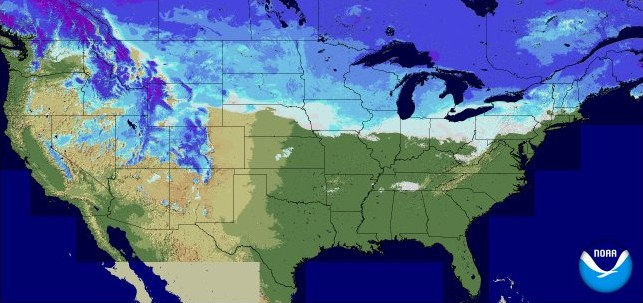
\includegraphics[width=\textwidth, trim= 0mm 0mm 0mm 0mm]{figs/snow_gt_1.jpg}
    \caption{January 1st, 2014}
    \label{fig:snow_map_gt_1}
  \end{subfigure}
  \begin{subfigure}[b]{0.33\textwidth}
    \centering
		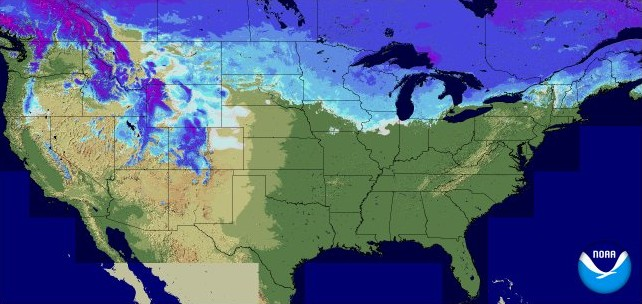
\includegraphics[width=\textwidth, trim= 0mm 0mm 0mm 0mm]{figs/snow_gt_2.jpg}
    \caption{January 15th, 2014}
    \label{fig:snow_map_gt_2}
  \end{subfigure}
  \begin{subfigure}[b]{0.33\textwidth}
    \centering
		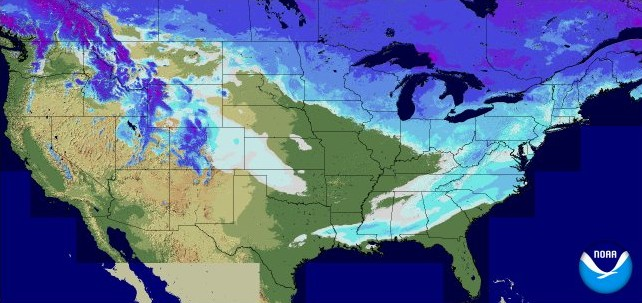
\includegraphics[width=\textwidth, trim= 0mm 0mm 0mm 0mm]{figs/snow_gt_3.jpg}
    \caption{January 29th, 2014}
    \label{fig:snow_map_gt_3}
  \end{subfigure}
  \begin{subfigure}[b]{0.33\textwidth}
    \centering
		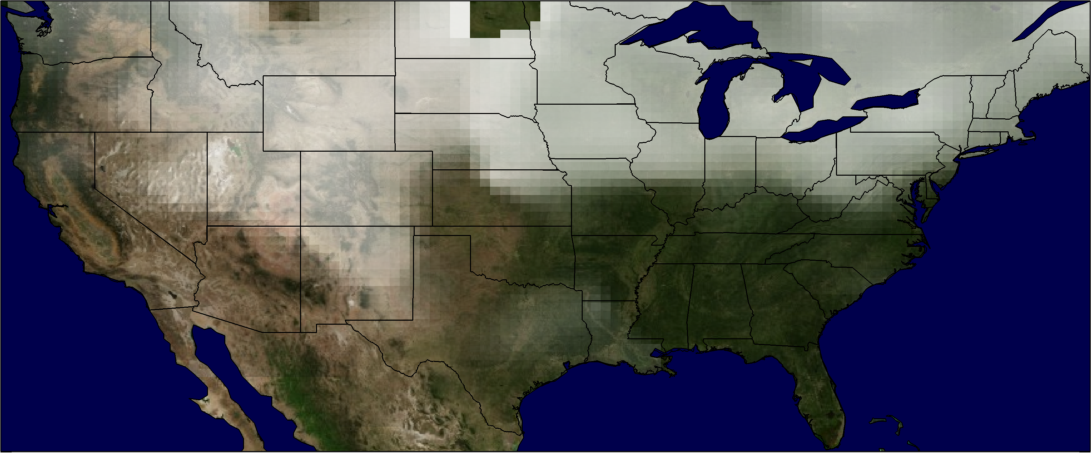
\includegraphics[width=\textwidth, trim= 0mm 0mm 0mm 0mm]{figs/snow_map_1.png}
    \caption{January 1st, 2014}
    \label{fig:snow_map_est_1}
  \end{subfigure}
  \begin{subfigure}[b]{0.33\textwidth}
    \centering
		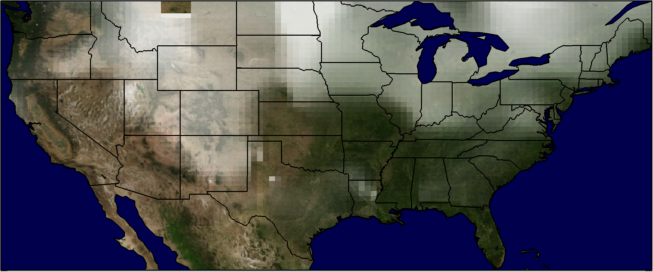
\includegraphics[width=\textwidth, trim= 0mm 0mm 0mm 0mm]{figs/snow_map_2.png}
    \caption{January 15th, 2014}
    \label{fig:snow_map_est_2}
  \end{subfigure}
  \begin{subfigure}[b]{0.33\textwidth}
    \centering
		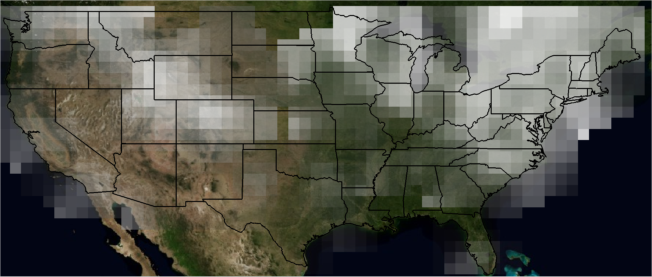
\includegraphics[width=\textwidth, trim= 0mm 0mm 0mm 0mm]{figs/snow_map_3.png}
    \caption{January 29th, 2014}
    \label{fig:snow_map_est_3}
  \end{subfigure}
  \caption{Maps of the \emph{snow} attribute from webcam data (bottom)
           across the continental United States in January 2014 and the
           corresponding map of snow depth created using remote 
           sensing data (top)~\cite{noaasite}.} 
  \label{fig:snow_maps}
\end{figure*}

To support rapid browsing of a large webcam image collection, we create
summaries of the transient attributes estimated by TransientNet.
\figref{webcam_summary} summarizes a year of images from AMOS webcams.
\figref{daylight} shows one year of the \emph{daylight} attribute,
\figref{clouds} shows one year of the \emph{clouds} attribute, and
\figref{snow} shows one year of the \emph{snow} attribute.  Each column in the
summary is a single day and each row a different time of the day (in 30 minute
intervals).  Each pixel is colored based on the attribute value for the
corresponding webcam image. Attributes such as \textit{snow}, \textit{cold},
and \textit{winter} have higher values in the winter months and lower values
during the summer months, as shown in \figref{snow}. The \textit{night} and
\textit{daylight} attributes clearly show the day/night cycle for the location
of the image, shown in \figref{daylight}.  Properties about the scene can be
inferred from these summaries.  Consistently high values for the
\textit{glowing} attribute at night indicate the presence of streetlights
and/or other man made light sources in the scene.  Such visualizations are more
robust to camera motion and more semantically meaningful than those based on
PCA~\cite{jacobs09webcamdata}.

\subsection{Mapping Weather Using Webcams}

\begin{figure}[t]
	\centering
		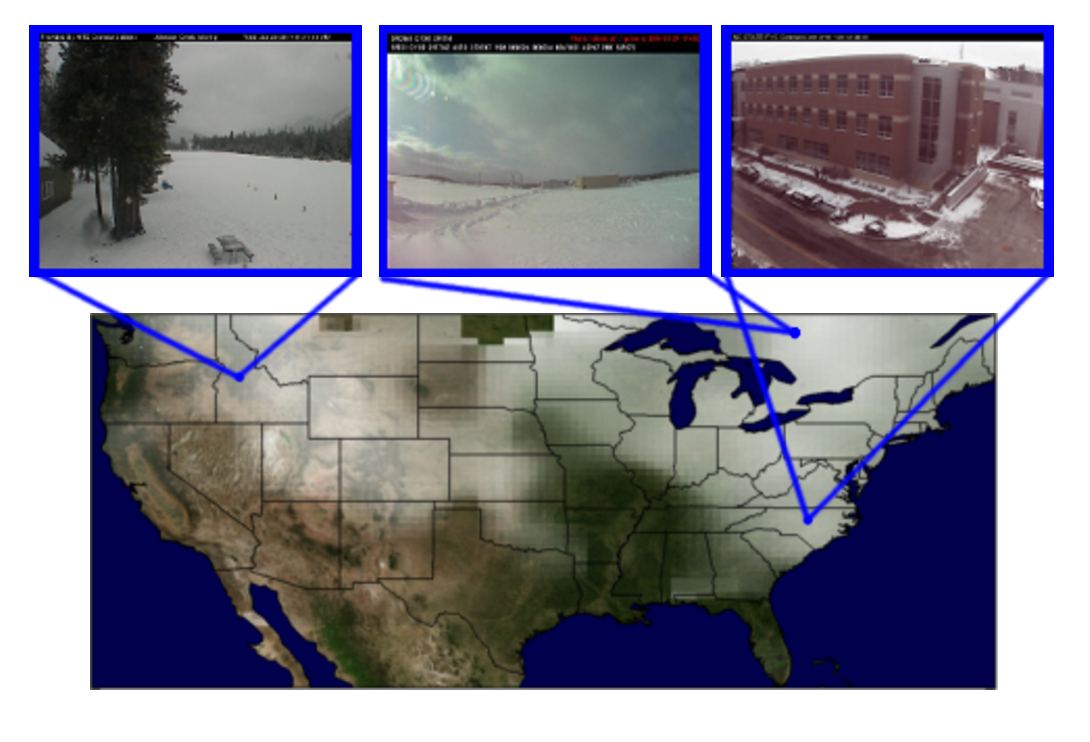
\includegraphics[width=0.5\textwidth, trim= 0mm 10mm 0mm 0mm]{figs/snow_exs.pdf}
		\caption{Snow map from \figref{snow_map_est_3} with three highlighted snowy 
             images.}
		\label{fig:snow_exs}
\end{figure}

We show how to use webcams with known locations to capture the geospatial
distribution of transient attributes. We downloaded data for January 2014 from
$3\,500$ AMOS webcams across the United States.  The images were labeled using
TransientNet-H to create a sparse distribution of points.  We then used locally
weighted averaging to estimate the attribute map.  This differs from the
technique proposed in Murdock et al.~\cite{murdock13clouds, murdock2015cloudmap}
in that our method uses a single model to make predictions for all cameras,
while Murdock et al.  create camera-specific models.

\figref{snow_maps} shows
three maps for the snow attribute across the continental United States.  Data
from January 2014 for AMOS webcams within the continental United States and the
southern edge of Canada was downloaded and labeled using TransientNet-H. These
maps show predicted snow coverage using only the \emph{snow} attribute.
Variation between the three maps shows snow accumulating and melting throughout
the month.  Anomalous regions of high snow values, such as those along the
California coast, come from false positive labels.  One such region comes from
a camera facing a white-sand beach, which appears visually similar to a snowy
scene.  Several cameras of this nature were manually pruned from the dataset.
\figref{snow_exs} shows example images from selected webcams on January 29th,
2014. The first two example images show heavy snow cover in northern areas and
the third example image shows the light snow cover in the south-eastern region
of the United States.  Maps for other attributes show expected natural
phenomena (the \textit{daylight} attribute increasing/decreasing east to west
as the sun rises/sets) and cues about the natural world (the \textit{rugged}
attribute higher in the mountainous west and low in the central plains).  

\subsection{Transient Semantics for Geolocalization}

Given a sufficient amount of time, the temporal pattern of the
transient attributes is a unique fingerprint of a location. We use
this observation and propose a robust method for geolocalizing outdoor
webcams. We adopt the framework of~\cite{jacobs07geolocate}, in which
the webcam location is found by relating temporal variations of
georegistered satellite imagery and the time series of features
extracted from webcam images. The estimated camera location is the
center of the satellite pixel for which the intensity is most
correlated with the webcam time series. The only change from the
original work is replacing the PCA coefficients (which are
unsupervised, but camera specific) with the transient attributes
(which are supervised, but not camera specific).

\begin{figure}[t]
  \centering
  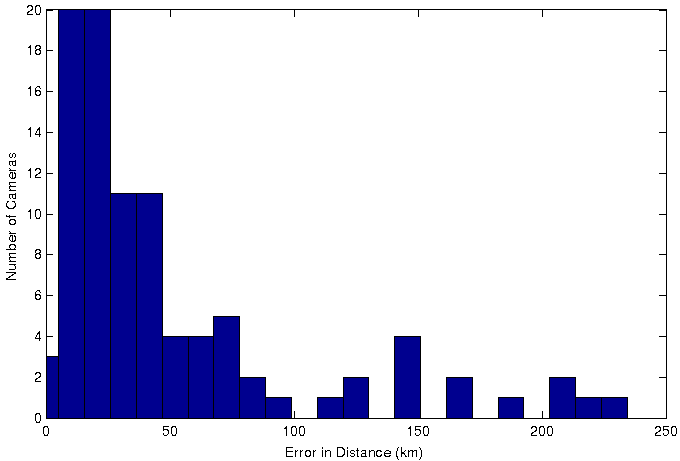
\includegraphics[width=.98\linewidth, trim= 20mm 0mm 20mm 0mm]{figs/geoloc/tran_errors}
  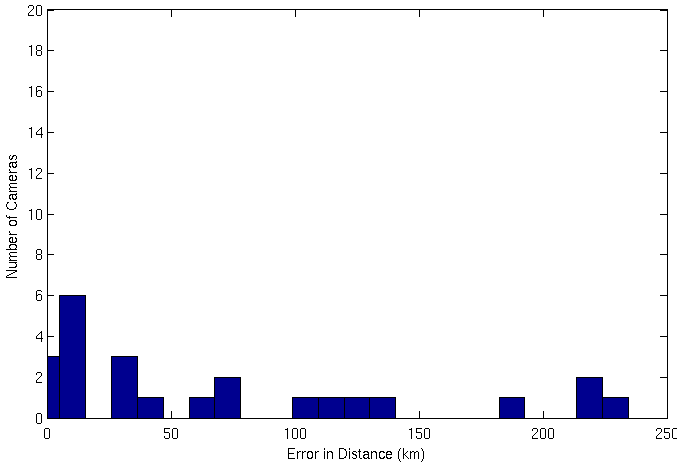
\includegraphics[width=.98\linewidth, trim= 20mm 0mm 20mm 0mm]{figs/geoloc/pca_errors}
  \caption{Webcam geolocalization errors for two methods. (top)
    Using the \textit{sunny} attribute. (bottom)
    Using the first PCA coefficient.}
  \label{fig:locerror}
\end{figure}

For evaluation, we downloaded a year (2013) of images from 180 randomly
selected webcams (\figref{webcamdist}) from the AMOS
dataset~\cite{jacobs07amos} and corresponding satellite
images~\cite{satimssite}.  We found that the \textit{sunny} attribute provided
the most accurate results and use it for all further figures. \figref{geoloc}
shows example correlation maps we estimated and \figref{locerror} shows the
evaluation results. Our method localizes 58\% of webcams within 250km from the
ground truth. As a baseline method, we repeated the experiment with the top 5
PCA coefficients. The best coefficient (the first) only locates 14\% of webcams
within 250km. We think the main advantage of using the transient attribute for
this task is that it is less sensitive to camera jitter, a significant problem
when applying PCA to outdoor webcam data. When the camera jitters it is likely
that the PCA coefficients encode for motion, not changes visible in satellite
imagery.

\begin{figure}[t]
	\centering
		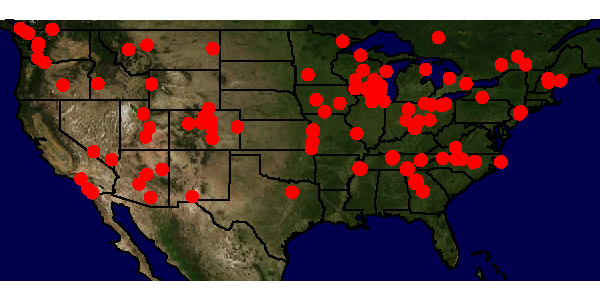
\includegraphics[width=0.5\textwidth, trim= 0mm 5mm 0mm 0mm]{figs/geoloc/webcam_dist}
		\caption{Distribution of webcams used in our geolocalization experiments.}
		\label{fig:webcamdist}
\end{figure}

\begin{figure}
	\centering
		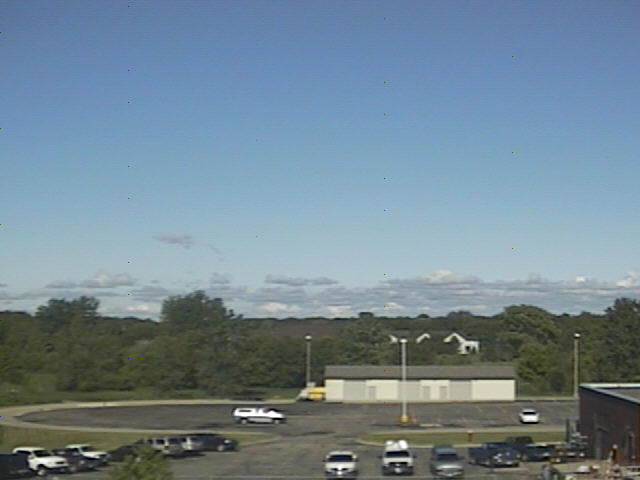
\includegraphics[width=0.18\textwidth]{figs/geoloc/297}
		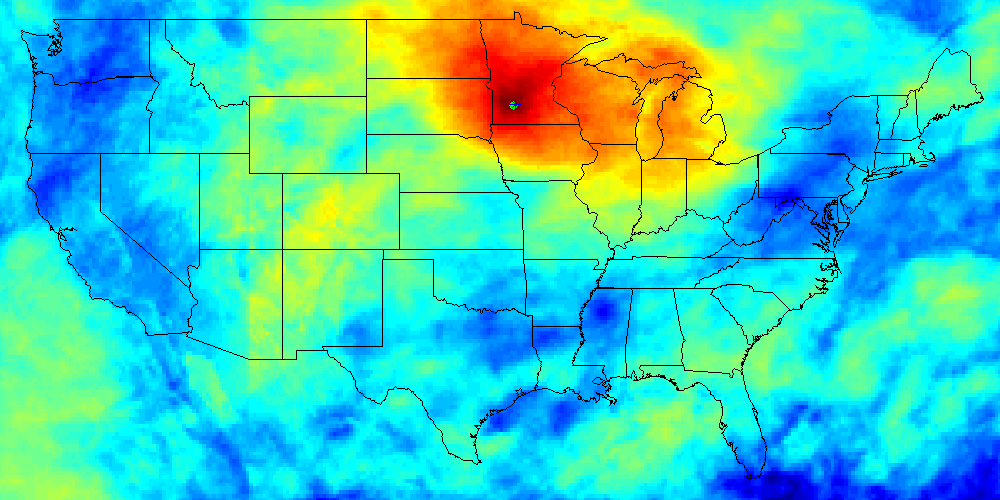
\includegraphics[width=0.27\textwidth]{figs/geoloc/geoloc_8_297}
		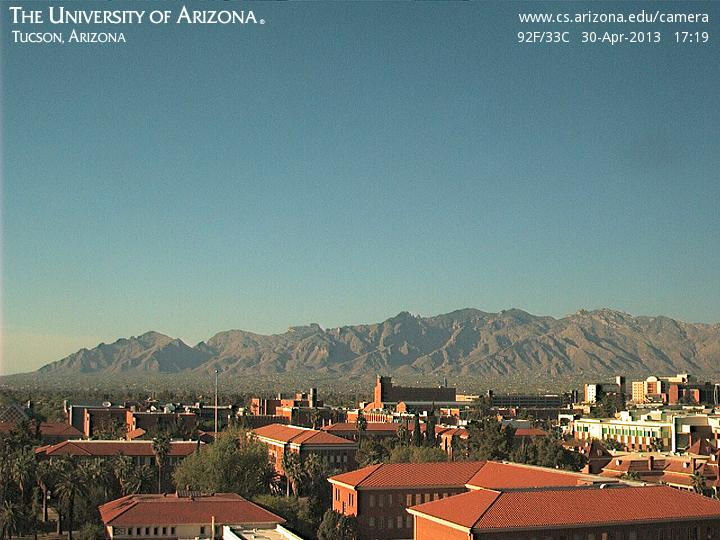
\includegraphics[width=0.18\textwidth]{figs/geoloc/5207}
		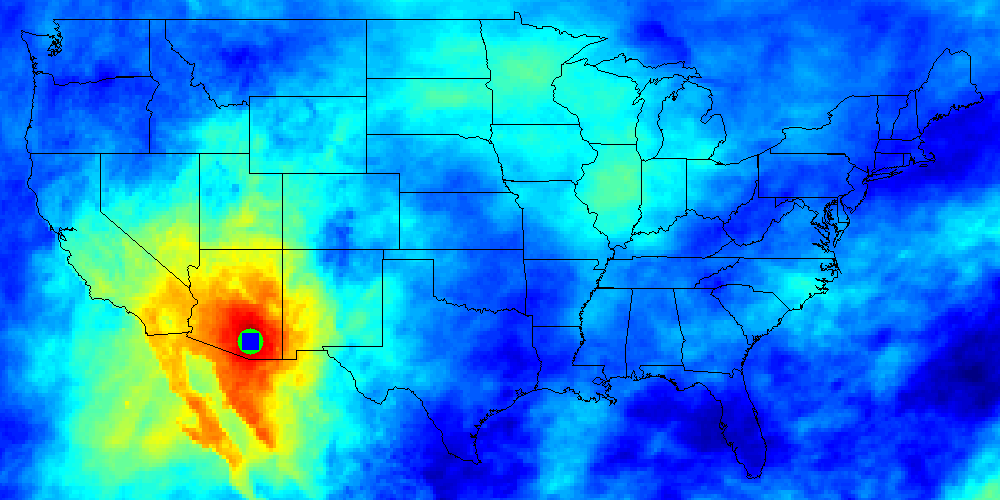
\includegraphics[width=0.27\textwidth]{figs/geoloc/geoloc_24_5207}
		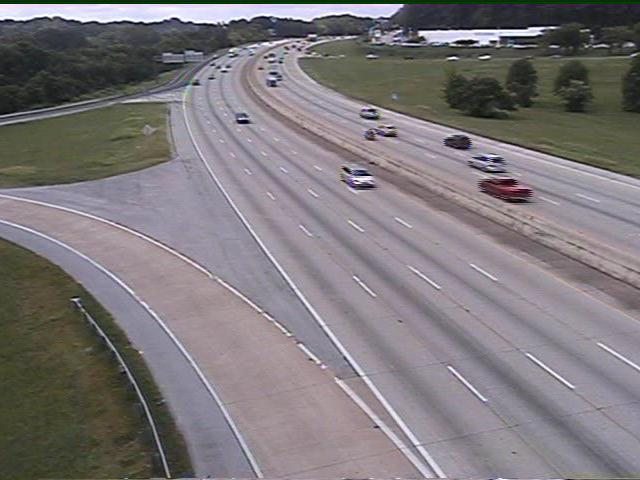
\includegraphics[width=0.18\textwidth]{figs/geoloc/23573}
		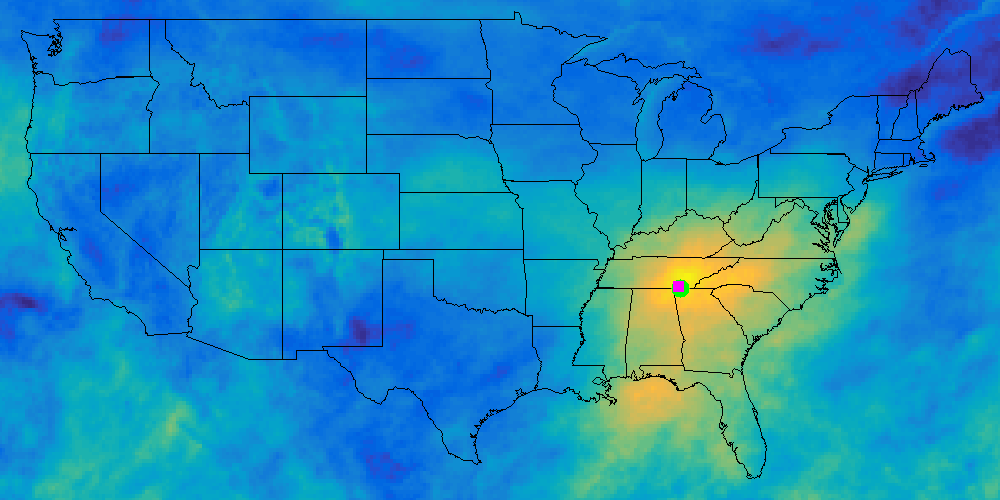
\includegraphics[width=0.27\textwidth]{figs/geoloc/geoloc_152_23573}
		\caption{Webcam geolocalization results using the
          \textit{sunny} attribute. (left) Webcam images and (right)
          estimated correlation maps, where orange 
          means more likely. Ground-truth locations are marked
          by green dots, predictions by blue squares.}
		\label{fig:geoloc}
\end{figure}

\section{Conclusions}

We introduced a fast method for predicting transient scene attributes
in a single image. Our method achieves state-of-the-art performance on
two benchmark datasets and requires no hand-engineered features, is
simple to train, and is very fast at test time. In addition, it can be
quickly extended to label additional attributes or adapted to new
datasets with a small amount of retraining. Together, these properties
make it particularly well suited to real-world applications, of which
we demonstrated several.

%The speed up
%provided by the CNNs allows us to predict transient scene properties for vast
%amounts of real-world data and propose several applications of the properties.
%We use this to label a large collection of webcam data and create year-long
%summaries for each webcam.  We also use a ``fully- convolutional'' network to
%show where attributes occur within an image.

%We introduce six deep convolutional neural networks for predicting transient
%scene attributes from a single image. These networks achieve state-of-the-art
%results on two benchmark datasets. The key advantages of the proposed approach
%are that it requires no hand-engineered features, is simple to train, is very
%fast at test time, and makes accurate predictions. In addition, these networks
%can be quickly extended to label additional attributes or adapted to new datasets
%with a small amount of retraining.  We demonstrate the real world
%ability of our methods for the task of automatically labeling outdoor
%webcams.
%
%In future work, we plan to explore the use of these networks in an
%application to micro-climate estimation from publicly available
%outdoor webcams~\cite{islam13webcamweather}. 

{\fontsize{8.5pt}{9.5pt}\selectfont
\bibliographystyle{ieee}
\bibliography{refs}
}

\end{document}
